%%
% Copyright (c) 2017, Pascal Wagler;  
% Copyright (c) 2014--2017, John MacFarlane
% 
% All rights reserved.
% 
% Redistribution and use in source and binary forms, with or without 
% modification, are permitted provided that the following conditions 
% are met:
% 
% - Redistributions of source code must retain the above copyright 
% notice, this list of conditions and the following disclaimer.
% 
% - Redistributions in binary form must reproduce the above copyright 
% notice, this list of conditions and the following disclaimer in the 
% documentation and/or other materials provided with the distribution.
% 
% - Neither the name of John MacFarlane nor the names of other 
% contributors may be used to endorse or promote products derived 
% from this software without specific prior written permission.
% 
% THIS SOFTWARE IS PROVIDED BY THE COPYRIGHT HOLDERS AND CONTRIBUTORS 
% "AS IS" AND ANY EXPRESS OR IMPLIED WARRANTIES, INCLUDING, BUT NOT 
% LIMITED TO, THE IMPLIED WARRANTIES OF MERCHANTABILITY AND FITNESS 
% FOR A PARTICULAR PURPOSE ARE DISCLAIMED. IN NO EVENT SHALL THE 
% COPYRIGHT OWNER OR CONTRIBUTORS BE LIABLE FOR ANY DIRECT, INDIRECT, 
% INCIDENTAL, SPECIAL, EXEMPLARY, OR CONSEQUENTIAL DAMAGES (INCLUDING,
% BUT NOT LIMITED TO, PROCUREMENT OF SUBSTITUTE GOODS OR SERVICES; 
% LOSS OF USE, DATA, OR PROFITS; OR BUSINESS INTERRUPTION) HOWEVER 
% CAUSED AND ON ANY THEORY OF LIABILITY, WHETHER IN CONTRACT, STRICT 
% LIABILITY, OR TORT (INCLUDING NEGLIGENCE OR OTHERWISE) ARISING IN 
% ANY WAY OUT OF THE USE OF THIS SOFTWARE, EVEN IF ADVISED OF THE 
% POSSIBILITY OF SUCH DAMAGE.
%%

%%
% For usage information and examples visit the GitHub page of this template:
% https://github.com/Wandmalfarbe/pandoc-latex-template
%%

\PassOptionsToPackage{unicode=true}{hyperref} % options for packages loaded elsewhere
\PassOptionsToPackage{hyphens}{url}
%
\documentclass[american,a4paper,oneside,,tablecaptionabove]{scrbook}
\usepackage{lmodern}
\usepackage{amssymb,amsmath}
\usepackage{ifxetex,ifluatex}
\usepackage{fixltx2e} % provides \textsubscript
\ifnum 0\ifxetex 1\fi\ifluatex 1\fi=0 % if pdftex
  \usepackage[T1]{fontenc}
  \usepackage[utf8]{inputenc}
  \usepackage{textcomp} % provides euro and other symbols
\else % if luatex or xelatex
  \usepackage{unicode-math}
  \defaultfontfeatures{Ligatures=TeX,Scale=MatchLowercase}
\fi
% use upquote if available, for straight quotes in verbatim environments
\IfFileExists{upquote.sty}{\usepackage{upquote}}{}
% use microtype if available
\IfFileExists{microtype.sty}{%
\usepackage[]{microtype}
\UseMicrotypeSet[protrusion]{basicmath} % disable protrusion for tt fonts
}{}
\IfFileExists{parskip.sty}{%
\usepackage{parskip}
}{% else
\setlength{\parindent}{0pt}
\setlength{\parskip}{6pt plus 2pt minus 1pt}
}
\usepackage{hyperref}
\hypersetup{
            pdftitle={Development of an interactive dashboard for performance reports on IBM Z systems with Linux},
            pdfauthor={Paul Bauriegel},
            pdfborder={0 0 0},
            breaklinks=true}
\urlstyle{same}  % don't use monospace font for urls
\usepackage[margin=2.5cm,includehead=true,includefoot=true,centering]{geometry}
\usepackage{listings}
\newcommand{\passthrough}[1]{#1}
\usepackage{graphicx,grffile}
\makeatletter
\def\maxwidth{\ifdim\Gin@nat@width>\linewidth\linewidth\else\Gin@nat@width\fi}
\def\maxheight{\ifdim\Gin@nat@height>\textheight\textheight\else\Gin@nat@height\fi}
\makeatother
% Scale images if necessary, so that they will not overflow the page
% margins by default, and it is still possible to overwrite the defaults
% using explicit options in \includegraphics[width, height, ...]{}
\setkeys{Gin}{width=\maxwidth,height=\maxheight,keepaspectratio}
\setlength{\emergencystretch}{3em}  % prevent overfull lines
\providecommand{\tightlist}{%
  \setlength{\itemsep}{0pt}\setlength{\parskip}{0pt}}
\setcounter{secnumdepth}{0}
% Redefines (sub)paragraphs to behave more like sections
\ifx\paragraph\undefined\else
\let\oldparagraph\paragraph
\renewcommand{\paragraph}[1]{\oldparagraph{#1}\mbox{}}
\fi
\ifx\subparagraph\undefined\else
\let\oldsubparagraph\subparagraph
\renewcommand{\subparagraph}[1]{\oldsubparagraph{#1}\mbox{}}
\fi

% Make use of float-package and set default placement for figures to H
\usepackage{float}
\floatplacement{figure}{H}

\usepackage{subfig}
\AtBeginDocument{%
\renewcommand*\figurename{Figure}
\renewcommand*\tablename{Table}
}
\AtBeginDocument{%
\renewcommand*\listfigurename{List of Figures}
\renewcommand*\listtablename{List of Tables}
}
\newcommand*\listoflistings\lstlistoflistings
\AtBeginDocument{%
\renewcommand*{\lstlistlistingname}{List of Listings}
}
\ifnum 0\ifxetex 1\fi\ifluatex 1\fi=0 % if pdftex
  \usepackage[shorthands=off,main=american]{babel}
\else
    % See issue https://github.com/reutenauer/polyglossia/issues/127
  \renewcommand*\familydefault{\sfdefault}
    % load polyglossia as late as possible as it *could* call bidi if RTL lang (e.g. Hebrew or Arabic)
  \usepackage{polyglossia}
  \setmainlanguage[variant=american]{english}
\fi

\title{Development of an interactive dashboard for performance reports on IBM Z
systems with Linux}
\providecommand{\subtitle}[1]{}
\subtitle{Term Paper T3000}
\author{Paul Bauriegel}
\date{}





%%
%% added
%%

%
% No language specified? take American English.
%


%
% colors
%
\usepackage[dvipsnames,svgnames*,x11names*,table]{xcolor}

%
% listing colors
%
\definecolor{listing-background}{HTML}{F7F7F7}
\definecolor{listing-rule}{HTML}{B3B2B3}
\definecolor{listing-numbers}{HTML}{B3B2B3}
\definecolor{listing-text-color}{HTML}{000000}
\definecolor{listing-keyword}{HTML}{435489}
\definecolor{listing-identifier}{HTML}{435489}
\definecolor{listing-string}{HTML}{00999A}
\definecolor{listing-comment}{HTML}{8E8E8E}
\definecolor{listing-javadoc-comment}{HTML}{006CA9}

%\definecolor{listing-background}{rgb}{0.97,0.97,0.97}
%\definecolor{listing-rule}{HTML}{B3B2B3}
%\definecolor{listing-numbers}{HTML}{B3B2B3}
%\definecolor{listing-text-color}{HTML}{000000}
%\definecolor{listing-keyword}{HTML}{D8006B}
%\definecolor{listing-identifier}{HTML}{000000}
%\definecolor{listing-string}{HTML}{006CA9}
%\definecolor{listing-comment}{rgb}{0.25,0.5,0.35}
%\definecolor{listing-javadoc-comment}{HTML}{006CA9}

%
% for the background color of the title page
%
\usepackage{pagecolor}
\usepackage{afterpage}

%
% TOC depth and 
% section numbering depth
%
\setcounter{tocdepth}{3}

%
% line spacing
%
\usepackage{setspace}
\setstretch{1.2}

%
% break urls
%
\PassOptionsToPackage{hyphens}{url}

%
% When using babel or polyglossia with biblatex, loading csquotes is recommended 
% to ensure that quoted texts are typeset according to the rules of your main language.
%
\usepackage{csquotes}

%
% captions
%
\definecolor{caption-color}{HTML}{777777}
\usepackage[font={stretch=1.2}, textfont={color=caption-color}, position=top, skip=4mm, labelfont=bf, singlelinecheck=false, justification=raggedright]{caption}
\setcapindent{0em}
\captionsetup[longtable]{position=above}

%
% blockquote
%
\definecolor{blockquote-border}{RGB}{221,221,221}
\definecolor{blockquote-text}{RGB}{119,119,119}
\usepackage{mdframed}
\newmdenv[rightline=false,bottomline=false,topline=false,linewidth=3pt,linecolor=blockquote-border,skipabove=\parskip]{customblockquote}
\renewenvironment{quote}{\begin{customblockquote}\list{}{\rightmargin=0em\leftmargin=0em}%
\item\relax\color{blockquote-text}\ignorespaces}{\unskip\unskip\endlist\end{customblockquote}}

%
% Source Sans Pro as the de­fault font fam­ily
% Source Code Pro for monospace text
%
% 'default' option sets the default 
% font family to Source Sans Pro, not \sfdefault.
%
\usepackage[default]{sourcesanspro}
\usepackage{sourcecodepro}

%
% heading color
%
\definecolor{heading-color}{RGB}{40,40,40}
\addtokomafont{section}{\color{heading-color}}
% When using the classes report, scrreprt, book, 
% scrbook or memoir, uncomment the following line.
%\addtokomafont{chapter}{\color{heading-color}}

%
% variables for title and author
%
\usepackage{titling}
\title{Development of an interactive dashboard for performance reports on IBM Z
systems with Linux}
\author{Paul Bauriegel}

%
% tables
%

%
% remove paragraph indention
%
\setlength{\parindent}{0pt}
\setlength{\parskip}{6pt plus 2pt minus 1pt}
\setlength{\emergencystretch}{3em}  % prevent overfull lines

%
%
% Listings
%
%

\lstdefinestyle{eisvogel_listing_style}{
  language         = java,
  numbers          = left,
  backgroundcolor  = \color{listing-background},
  basicstyle       = \color{listing-text-color}\small\ttfamily{}\linespread{1.15}, % print whole listing small
  xleftmargin      = 2.7em,
  breaklines       = true,
  frame            = single,
  framesep         = 0.6mm,
  rulecolor        = \color{listing-rule},
  frameround       = ffff,
  framexleftmargin = 2.5em,
  tabsize          = 4,
  numberstyle      = \color{listing-numbers},
  aboveskip        = 1.0em,
  keywordstyle     = \color{listing-keyword}\bfseries,
  classoffset      = 0,
  sensitive        = true,
  identifierstyle  = \color{listing-identifier},
  commentstyle     = \color{listing-comment},
  morecomment      = [s][\color{listing-javadoc-comment}]{/**}{*/},
  stringstyle      = \color{listing-string},
  showstringspaces = false,
  escapeinside     = {/*@}{@*/}, % Allow LaTeX inside these special comments
  literate         =
  {á}{{\'a}}1 {é}{{\'e}}1 {í}{{\'i}}1 {ó}{{\'o}}1 {ú}{{\'u}}1
  {Á}{{\'A}}1 {É}{{\'E}}1 {Í}{{\'I}}1 {Ó}{{\'O}}1 {Ú}{{\'U}}1
  {à}{{\`a}}1 {è}{{\'e}}1 {ì}{{\`i}}1 {ò}{{\`o}}1 {ù}{{\`u}}1
  {À}{{\`A}}1 {È}{{\'E}}1 {Ì}{{\`I}}1 {Ò}{{\`O}}1 {Ù}{{\`U}}1
  {ä}{{\"a}}1 {ë}{{\"e}}1 {ï}{{\"i}}1 {ö}{{\"o}}1 {ü}{{\"u}}1
  {Ä}{{\"A}}1 {Ë}{{\"E}}1 {Ï}{{\"I}}1 {Ö}{{\"O}}1 {Ü}{{\"U}}1
  {â}{{\^a}}1 {ê}{{\^e}}1 {î}{{\^i}}1 {ô}{{\^o}}1 {û}{{\^u}}1
  {Â}{{\^A}}1 {Ê}{{\^E}}1 {Î}{{\^I}}1 {Ô}{{\^O}}1 {Û}{{\^U}}1
  {œ}{{\oe}}1 {Œ}{{\OE}}1 {æ}{{\ae}}1 {Æ}{{\AE}}1 {ß}{{\ss}}1
  {ç}{{\c c}}1 {Ç}{{\c C}}1 {ø}{{\o}}1 {å}{{\r a}}1 {Å}{{\r A}}1
  {€}{{\EUR}}1 {£}{{\pounds}}1 {«}{{\guillemotleft}}1
  {»}{{\guillemotright}}1 {ñ}{{\~n}}1 {Ñ}{{\~N}}1 {¿}{{?`}}1
  {…}{{\ldots}}1 {≥}{{>=}}1 {≤}{{<=}}1 {„}{{\glqq}}1 {“}{{\grqq}}1
  {”}{{''}}1
}
\lstset{style=eisvogel_listing_style}

\lstdefinelanguage{XML}{
  morestring      = [b]",
  moredelim       = [s][\bfseries\color{listing-keyword}]{<}{\ },
  moredelim       = [s][\bfseries\color{listing-keyword}]{</}{>},
  moredelim       = [l][\bfseries\color{listing-keyword}]{/>},
  moredelim       = [l][\bfseries\color{listing-keyword}]{>},
  morecomment     = [s]{<?}{?>},
  morecomment     = [s]{<!--}{-->},
  commentstyle    = \color{listing-comment},
  stringstyle     = \color{listing-string},
  identifierstyle = \color{listing-identifier}
}

%
% header and footer
%
\usepackage{fancyhdr}
\pagestyle{fancy}
\fancyhead{}
\fancyfoot{}
\lhead{Development of an interactive dashboard for performance reports on IBM Z
systems with Linux}
\chead{}
\rhead{}
\lfoot{Paul Bauriegel}
\cfoot{}
\rfoot{\thepage}
\renewcommand{\headrulewidth}{0.4pt}
\renewcommand{\footrulewidth}{0.4pt}

%%
%% end added
%%

\begin{document}

%%
%% begin titlepage
%%

\begin{titlepage}
\newgeometry{left=6cm}
\definecolor{titlepage-color}{HTML}{25467a}
\newpagecolor{titlepage-color}\afterpage{\restorepagecolor}
\newcommand{\colorRule}[3][black]{\textcolor[HTML]{#1}{\rule{#2}{#3}}}
\begin{flushleft}
\noindent
\\[-1em]
\color[HTML]{ffffff}
\makebox[0pt][l]{\colorRule[ffffff]{1.3\textwidth}{1pt}}
\par
\noindent

{ \setstretch{1.4}
\vfill
\noindent {\huge \textbf{\textsf{Development of an interactive dashboard for performance reports on IBM Z
systems with Linux}}}
\vskip 1em
{\Large \textsf{Term Paper T3000}}
\vskip 2em
\noindent
{\Large \textsf{\MakeUppercase{Paul Bauriegel}}
\vfill
}

\textsf{}}
\end{flushleft}
\end{titlepage}
\restoregeometry

%%
%% end titlepage
%%



\pagestyle{plain}
\pagenumbering{Roman}

{
\setcounter{tocdepth}{2}
\tableofcontents
}

\pagestyle{fancy}
\pagenumbering{arabic}
\setcounter{page}{1}
\chapter{Introduction}\label{introduction}

Data is a valuable resource (1), especially when analyzing or comparing
the performance of different technologies. With test data, it's possible
to find bottlenecks in applications or errors in the process flow.
However, most large data set are useless until there have been evaluated
or visualized to gain insights. The visualization makes it easier for
the analyst to understand the relations and evolutions inside the data.
As result, it makes his work more efficient. Nevertheless, visualization
takes valuable time, especially when it has to be done over and over
again. There are several software solutions on the market
{[}Meek.2017{]} to automate these visualizations and get fast insights,
like \emph{Tableau} or \emph{Voyager 2} (2). But there are also
circumstances which require highly customized reports, as it is
necessary for the \emph{IBM z Linux Performance} department.\\
The \emph{IBM z Linux Performance} department has several test
procedures to evaluate the IBM Z Mainframes on Linux for several
workloads. These test runs result in different kinds of reports. By now
these reports had to be manually analyzed. The goal of this project is
to support the performance analysists by creating an interactive
dashboard for their requirements. The dashboard aims to automate the
process of visualization without losing the flexibility in the data
presentation.

This paper presents a working dashboard with specialized performance
visualizations. It discusses the design choices for technology and
architecture in this application and the ideas behind the different
visualizations. The report highlights the advantages of this tool as
well as further challenges.

Therefore the reader will be introduced to the design aspects of data
visualization and the requirements for an interactive performance
visualization dashboard. The first chapter explains how effective data
visualization has to be implemented. The second provides a case study
for the application, which includes detailed information about the data
source.\\
On this foundation, the technologies and architecture of the application
will be explained. The part compares the different technology options
and underlines the design decisions.\\
Based on the architecture the dashboard prototype will be explained and
which further improvements could be implemented.

\chapter{Concepts of data
visualization}\label{concepts-of-data-visualization}

\section{What means data
visualization}\label{what-means-data-visualization}

Visualization meant in its original sense to \enquote{construct a visual
image in the mind} (3). In the computer science the understanding for
this term is different, as Earnshaw defines it:\\
\enquote{Scientific Visualization is concerned with exploring data and
information in such a way as to gain understanding and insight into the
data.} (4)\\
The term is now referring to building a visual image based on data. Or
in a generalized context, it means data visualization. There are
multiple definitions for the term data visualization on different levels
of abstraction (5). In the words of Ignatius and Senay:\\
\enquote{The primary objective in data visualization is to gain insight
into an information space.} (6)\\
Data visualization has varieties like in information or scientific
visualization {[}Friendly{]}. These terms have a slightly different
semantical definition. Information visualization is more precise because
it presents the data in a specific interpretation context (7). The term
scientific visualization is mostly used in the context of visualization
for science research (4). Because the distinction is not relevant for
this paper, the terms will be used equally in the further chapters.\\
The dashboard described in this paper is a tool for information
visualization. Therefore information visualization will be described
shortly. According to Gershon information visualization
\enquote{combines aspects of scientific visualization, human-computer
interfaces, data mining, imaging and graphics} (8).\\
Information visualization has two main goals (9):

\begin{itemize}
\item
  data representation, by transferring the data in a suitable layout for
  presentation
\item
  data exploration or visual data mining meaning the discovery of new
  knowledge by transforming and interconnecting the data.
\end{itemize}

The data representation should allow to find and view the data on
specific criteria. The representation should contain multiple views on
the selection with a different context. The representation easy to keep
in mind, to support the analyst.\\
The data exploration should highlight relations and structures in the
data. To find insights multiple data sets should be interconnect-able.
(10)

\section{The process of data
visualization}\label{the-process-of-data-visualization}

Russell Ackoff defines the process of discovering new knowledge in three
abstract levels for the perceptual and cognitive space (11). The paper
by Chen et al. extends these definitions for the computational space
(12). These levels are:\\
Data - Data is a concatenation of different symbols, for example to
strings. In the computer science, data can by any stored representations
of models or attributes in the memory.\\
Information - Information is processed data that has been given a
context. The context can be assigned by either a computational process
or humans annotating the data.\\
Knowledge - Knowledge is an application of data and information to
understand the processes and developments that created the data. This
can be the results of a machine learning process or analysis by subject
matter experts.\\
Understanding - Understanding extends the knowledge by providing
explanations for the developments in the data.

\begin{figure}
\centering
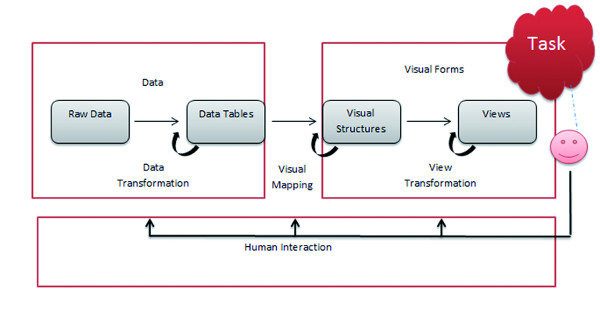
\includegraphics[width=0.50000\textwidth]{images/krypczyk_diagrammarten_1.jpg}
\caption{Process of visualization}
\end{figure}

The process of visualization has been defined in a reference model by
Card, Mackinlay, and Shneiderman (13). The model has three
transformation phases, to transform the data between the different
levels of knowledge. The process begins with the raw data being
transformed into structured tables. Data in tabular form is easier to
visualize. The \emph{data} becomes \emph{information}.\\
The visual mapping converts the data tables into visual structures.
These have graphical properties instead of the mathematical relation
inside the tables. The mapping into structures results in possible
\emph{knowledge} for the viewer. Such a mapping depends on the chosen
chart type and if the data is discrete or continuous.\\
In the last transformation step, the visualization is adjusted to
highlight parts of the data and get a better \emph{understanding}. On a
user-driven dashboard, the user \textbf{interacts with the
visualization} to create different views.

The model has also been refined by dos Santos (15), adding new data
filtering step after the general data transformations. In the option of
the author this model over specified for most modern use cases, where
big data sets are evaluated in real time and can be filtered in the
frontend. Furthermore, the model is specialized on generating images.
When the visualization is rendered for example on the server side this
model is applicable, but in a modern visualization frontend, the
visualization doesn't have to be a picture or in Ben Shneiderman's
words: \enquote{The purpose of visualization is insight, not pictures.}
(13)

\section{Visualization best
practices}\label{visualization-best-practices}

In an interactive dashboard, the user can adjust his view of the data,
but not the kind of representation. The representation type is stills
defined in the visual structures. Best practices for visualization help
to develop an appealing visual mapping of the data. The chapter
summarizes the Graphical excellence points laid out by Edward Tufte (16,
p.~13, 17).

\emph{Show the complete data} - Provide the data source, with its
limitations\\
\emph{Data over Visualization} - Encourage the viewer to think about the
substance rather than it's representation or methodology\\
\emph{Assume an Intelligent Audience} - Don't oversimplify the data or
the visualization, induce the viewer to think about the data\\
\emph{Encourage data exploration} - show the data at several levels of
detail, from broad overview to the fine structure, enable comparisons
for different pieces of data\\
\emph{Make data understandable} - integrate verbal descriptions in the
dataset, avoid distorting what the data have to say and follow
conventions when presenting the data.\\
\emph{Avoid confusing charts} - choosing the wrong representation can
unintentionally confuse or deliberately mislead the viewer.

\section{Choosing the best chart
type}\label{choosing-the-best-chart-type}

How easily the user is able to work with the data depends mainly on the
type of chart. Mackinlay and Tufte use their publication to explain
their selection of visualization type based on sets of examples. This
paper will not summarize their main works. Instead, it will use simple
classifications guidelines for the choice of visualization. To decide if
either a chart or another representation is used, the Visual Thinking
Codex by Dan Roam will be applied. This paper expects that all data will
be represented as a chart. Because of that a chart selection diagram by
Andrew Abela should help to use the best chart visualization (18).

The Visual Thinking Codex is a tool for visual thinking by Dan Roam
(19). Visual thinking is a methodology to organize the thoughts by
visualizing them. The codex is using another tool called SQVID. The idea
behind SQVID is that you can think of a thing in a variety of different
ways. \textbf{S}imple or Elaborate, \textbf{Q}ualitative vs
Quantitative, \textbf{V}ision and Execution, \textbf{I}ndividual against
Comparison, \textbf{D}ifference/change or As is. (20)\\
The codex suggests different types of visualization. The decision is
based on the question that should answer and kind focus on covered by
the SQVID methodology.\\
Any z performance analyst asks primarily two kinds of question
\emph{How} is sth. and \emph{Why} is it like this. For example
\emph{How} much memory is used?, or \emph{Why} are we losing
performance?. These questions come from different view angles so that no
filtering based on the kind thinking can be made. But on the questions
only it can be seen that plots and charts are the primary visualization
type. Therefore a further chart study can provide some advice for
choosing the right chart. (19)

As part of the Extreme Presentation \textsuperscript{TM} Method, Abela
did provide a Chart Suggestion graphic which can help to choose the
right presentation method. The main question is what should be shown. A
comparison can be shown in bar or column charts. Distribution may be
better with histograms. A relationship requires a bubble or scatter
chart and a composition can be shown with stacked or pie charts. This
source is just meant to be a simple overview and is not in any meaning
complete. (18)

Good resources (21) for a more detailed exploration of graphs are the
following. For the fundamentals of graph design \enquote{Show Me the
Numbers} by Stephen few is a helpful resource. The best encyclopedic
reference for visualization is \enquote{Information Graphics} by Robert
Harris. For an even more detailed exploration of visualization
\enquote{The Visual Display of Quantitative Information} by Edward (16)
and \enquote{The Elements of Graphing Data} by William Cleveland can be
used.\\
The \enquote{perception edge} blog (22) provides a collection of
different papers, with solutions for more or less common problems when
developing chart. Some of these suggestions will be used in the further
implementation.

\chapter{Use case study of the application
requirements}\label{use-case-study-of-the-application-requirements}

Building a good visualization is not easy. To build a helpful
visualization this chapter will introduce design principles, processed
and an overview how the actual data looks like. This information should
help to develop a dashboard on the needs of the user and with the right
processes or technologies.

\section{Use Case Analytics with User Experience
principles}\label{use-case-analytics-with-user-experience-principles}

Choosing a matching visualization type makes the data understandable.
According to Tufte good graphics are furthermore encouraging the viewers
also to explore the dataset. Therefore this paper is proposing an
interactive dashboard. To ensure the best user experience on the
dashboard, this chapter will introduce the User Interface (UI) Design
and User Experience (UX) Design. In simple words is UI how things
\textbf{look} and UX how things \textbf{work}. (23) This chapter will
outline the main UI design principles and which UX processes help to
develop the best user experience.

\subsection{UI design principles}\label{ui-design-principles}

Good UI design and suitable design principles have been defined by many
authors over the time. The paper will cite three publications on a
different degree of details. At first, the main principles of design
will be presented based on the Donald Normans book \enquote{The Design
of Everyday Things}. Than these principles will be specialized for the
UI design. At last, the principles of website design will be explained
based on \enquote{Don't Make Me Think} by Steve Krug.

Thinking about the design of a product before building it, results in
more user-friendly products. Norman provides seven principles, which
good designers should follow.

\emph{Provide the Necessary Knowledge} - The user builds his own
conceptual model how the thing is working. Good design provides the
information to interpret and understand the object. It contains visible
clues for their function.\\
\emph{Simplify} - The complexity of the product increases as the square
of the features. To simplify tasks four methods can be used. Provide the
user a simple, intuitive mental aid. Show feedback to the user instead
of making they remembering things. Third and Fourth, automate functions
and change the way of presenting the information.\\
\emph{Show How to Use a Tool and Explain Its State} - The user should
know about the consequences of their actions and the devices gave them
feedback promptly.\\
\emph{Map Correctly} - Developing a product should consider the user's
natural mappings (e.g. \enquote{up} more naturally suggests
\enquote{louder} than does \enquote{left})\\
\emph{Use Constraints} - Contains help to understand the product. The
lead the user to use the product in the correct way.\\
\emph{Expect Errors} - If the user can create an error, it's very likely
he will do so. Good design prevents as many errors as possible and gives
informative feedback, for those that cannot be prevented. Most errors
are either \enquote{slips} or \enquote{mistakes.} Slips are errors by
accident, like throwing the wrong document in the trash. Mistakes, on
the other hand, are conscious actions, taken by having the wrong goal or
misleading information.\\
\emph{Consider Standardizing} - Standardization is useful because they
base your application on a ground of common knowledge for all user.
Consider a car, wherever on the word you take a car, there are all
operating same way.

For User Interfaces, the core practices concentrate more on the style
aspects of the application. There five key principles a good UI is
measured on (24).\\
\emph{Color} - The color is influencing the emotions of the viewer. Some
meanings of colors are predefined like red for attention. Knowing about
the psychology of colors is important. Principles of color do also
include using matching color schemes for charts or web elements. (25)\\
\emph{Balance} - Balance in the design context is arranging elements to
establish a positive communication to the user. Getting the interest and
positive feedback by the user is achieved by multiple criteria, like
symmetry, asymmetry, or alignment. (26)\\
\emph{Contrast} - Contrast is used for three main reasons. 1. Contrast
is attractive to the eye, 2. It helps to organize information or build a
hierarchy, 3. The Contrast moves elements in the focus of the viewer.
(27)\\
\emph{Typography} - Fonts and the content itself are the main influence
how users process the given information. Therefore the should be chosen
with caution. (28)\\
\emph{Consistency} - Consistency is the key principle in UI design. It
makes the product intuitive, usable and eliminates confusion.
Consistency is based on familiar patterns and common visuals like color
schemes, same typography or spaces between elements. (29)

This work will create a User Interface for a web-application as
explained further in chapter sec.~\ref{sec:frontend-req}. Steven Krug
did summarize the key principles for website Design in his book. To get
a basic understanding of good website design his core point will here be
summarized.

\emph{Create a clear visual hierarchy} -- As defined by consistency
principle the web page should \enquote{clearly and accurately portray
the relationships among the things on the page.}. If elements are
conceptually linked, they are visually linked as well. Important aspects
are highlighted with visual cues, like bold or larger fonts.\\
\emph{Take advantage of conventions} -- \emph{Standardizations} in web
pages make use their conventions. This can recognizable icons, like a
person for the login profile or design languages like Material Design
for the webpage.\\
\emph{Break up pages into clearly defined areas} -- Create different
views for every independent context.\\
\emph{Make it obvious what's clickable} -- People click when using a
website. The indication of clickable items and action make it easier for
the user to understand \emph{how to use the tool}\\
\emph{Minimize noise} -- To avoid distractions on the web interface
remove anything that draws the users away from your focus.

\subsection{User Experience processes}\label{user-experience-processes}

In contrast to the UI Design, the User Experience Design is a creative
process to find the best design by analyzing the user (30). It helps the
business to define the brand image, based on the target group. The sales
and the site traffic are increasing because the users enjoy the product.
And in general, UX establishing customer loyalty and goodwill (31).

Good User Experience has three primary descriptions: Useful, Usable,
Delightful. Useful means that the solution is matching all user needs,
also the need they might not be aware of. Usable describes the product
to be easy to use and intuitive, the user needs no concentration for the
basic functions. Delightful is your interface or product if the user
enjoys it. It motivates the user to work with it.

Every UX design process has some common features, which will be
explained shortly. These steps help to develop a great user experience.
Therefore these processes are used while developing the dashboard.
(32)\\
The first step of each UX workflow is research (33). This step is about
requiring data and thinking about to user. Based on this data different
group of people sharing similar goals can be distinguished.\\
Here starts the UX Analysis, also called UX Strategy (34). In this part,
the data about persons brought in some context. These groups are bundles
into a Persona. A persona contains the behaviors, interests, and goals
for a user group (35). The persona is then extended with user stories
and scenario maps. The user story describes from the users perspective
what the product should accomplish or how it should be working (36). In
extension, a scenario map is built. The scenario map is analyzing the
step a user will take to accomplish a given task (37). Based on the
concrete UX methodology further analysis is done.\\
When the UX Analysis is completed, the actual UX Design starts. This
includes building a variety of different Wireframes to build Interaction
Prototypes for the best ideas. Good design means in UX not automatically
good aesthetics. Actually, aesthetics has the lowest priority in the
product design, more important is a consistent, structured and
understandable layout (38).\\
Finally, the UI implementation will be done and delivered to test and
validate the design. Therefore metrics and analytics tools are used to
track how the users use our product and how satisfied there are.\\
To achieve good user experience many companies use a specific
methodology. Very popular are Design Thinking (39) or the Double Diamond
(40) process. IBM is using a modified version of Design Think called IBM
Design Thinking (41).

\section{Use case study of the data source}\label{sec:usecase-dat}

All reports are stored in one server directory which the visualization
dashboard has access to. The data storage contains reports of different
kinds. These reports contain monitored performance data for IBM Z
systems on Linux. This section provides a short overview about the raw
data formats, that can be visualized by the application stack. This is
four different formats: System Activity Report reports for Linux,
profiling binary data and graphviz files in general, textual log files
in a specific format and internal reports for processing units.

The System Activity Reports are collected by a Linux tool called
\emph{sar}. \emph{Sar} is part of the \emph{sysstat} package. Sysstat is
a collection of performance monitoring tools maintained by Sebastien
Godard. The sar command line utility collects multiple datasets, most
important of which are the activity of CPU, transfer rates of the disk
or utilization of memory. A complete list of collected data can be
gathered from the sar manual (42). The resulting data is stored in three
formats, in textual data (sartxt), tabular CSV data (sarcsv) and in JSON
form (sarjson). The application works with the sarcsv data :

\begin{lstlisting}[caption={Sysstat report - sarcsv file}]
# hostname;interval;timestamp;CPU;%usr;%nice;%sys;%iowait;%steal;%irq;%soft;%guest;%gnice; %idle
r72klaus;10;2017-12-21 12:24:34 UTC;-1;63.88;0.00;24.48;0.00;0.01;0.24;9.14;0.00;0.00;2.25
r72klaus;10;2017-12-21 12:24:34 UTC;0;63.44;0.00;25.77;0.00;0.00;0.20;8.19;0.00;0.00;2.40
...
# hostname;interval;timestamp;proc/s;cswch/s
r72klaus;10;2017-12-21 12:24:34 UTC;13.60;399407.80
r72klaus;10;2017-12-21 12:24:44 UTC;1.10;391299.20
....
\end{lstlisting}

Sar is an often used tool for performance monitoring in Linux. Because
of that, there exist multiple visualization tools, which can be used to
get visualization inspirations.\\
In contrast to the other report formats the sar files are increasing in
size based on the runtime of the test. In some test cases the files can
grow up to hundred's of megabyte.

The programs running on IBM Z are also profiled by different profiling
tools, such as perf or gprof. The application is analyzing these reports
by its self. The application stack makes use of an existing
visualization program developed by Jose Fonseca called gprof2dot. The
tool can handle the data from all popular profiling tool for C, Python
or Java. This tool return graphs in the graphviz dot format. The
application should render these graphs.

The textual log report have a special naming conversion and marker for
the relevant data inside. The naming convention distinct's them from
normal text files. The log files have the following syntax:

\begin{lstlisting}[caption={Logfile for Tensorflow tests}]
WARNING:tensorflow:Using temporary folder as model directory: /tmp/tmp6bU9WX
2017-12-11 17:37:38.556092: I tensorflow/core/platform/cpu_feature_guard.cc:137] Your CPU supports instructions that this TensorFlow binary was not compiled to use: AVX512F
...
###START### REAL:0.000411033630371 CPU:0.000412
Total words: 7664
...
###PREPARE### REAL:2.52717900276 CPU:2.520947
###TRAIN### REAL:248.245265961 CPU:383.199024
...
\end{lstlisting}

The fourth format for the processing unit reports (PU Report) is yet
another log format. One log files contain about a hundred headers for
data that are commonly in tabular form.

\section{Current visualization workflow for the performance
analysts}\label{current-visualization-workflow-for-the-performance-analysts}

At the point of this paper, a web application for browsing performance
data existed. This work was based on the idea of visualizing all the
data that can be accessed by this application.\\
The current application has only some basic features. It provides a
login page, which provides a protection for all other pages. These pages
where static web pages like a documentation site and a dynamic view for
a server directory to download files.\\
To visualize the performance reports, they have to be downloaded and
then externally visualized. The data often needs to be pre-processed by
some script before the visualization.\\
Visualizing the reports directly in the current application would
simplify the visualization workflow. It makes the pre-processing
unnecessary and creates a data-driven visualization automatically. This
is speeding up thing and help the users to focus on the real problems.

\section{Results of the use case analysis - What are the requirements
for the dashboard.}\label{sec:usecase-result}

This chapter will summarize the information, goals and wishes for the
application gathered by the processes described before. These
information contain technical requirements as well as abstract ideas for
the application.

\begin{enumerate}
\def\labelenumi{\arabic{enumi}.}
\tightlist
\item
  The dashboard should be a working prototype, which can visualize
  multiple kinds of reports. The visualizations for the reports should
  contain multiple views based on the data sets.
\item
  It should extend the existing application for browsing the web
  directories. There is no need to develop a independent application.
\item
  The dashboard should works on a diversity of devices used in the
  department. A platform independent solution should be intended, since
  multiple operating systems and browser are used by the people. The
  main platform is Desktop not Mobile.
\item
  The user can dynamically interact with the visualizations. The
  visualisation are commonly charts, some of them could be graphs as
  well. The charts should be configurable, like setting the scale or
  enabling gridlines. The chart should also react on mouse interactions,
  like showing tooltips or more specific charts.
\item
  The interface has short loading times even with the larger report
  files. A common use case would be to just take a short look into the
  file, therefore only the necessary data should be transmitted to the
  client.
\item
  The timeframe for the implementation are seven weeks. The project
  should focus on some core features and the existing code basis should
  be reused.
\item
  The work should be documented in the source code with comments and by
  this paper.
\end{enumerate}

\chapter{Architecture decisions based on the use
case}\label{architecture-decisions-based-on-the-use-case}

In the previous chapter, the ideas and goals for the new dashboard had
been collected. This chapter will discuss how these ideas determine the
architecture of the application. This chapter will also define the
requirements for the technologies based on the architecture and the
goals for the application.

\section{Architecture overview to achieve the application
goals}\label{architecture-overview-to-achieve-the-application-goals}

The dashboard application will continue using the two-tier architecture.
The primary reason for this architecture decision is the simple handling
of users and files (43). The server part can handle access and provision
of the files. The client visualizes the data for the user. Which options
of splitting the visualization pipeline are possible discusses the
graphic by Tominski shown below (44).

\begin{figure}
\centering
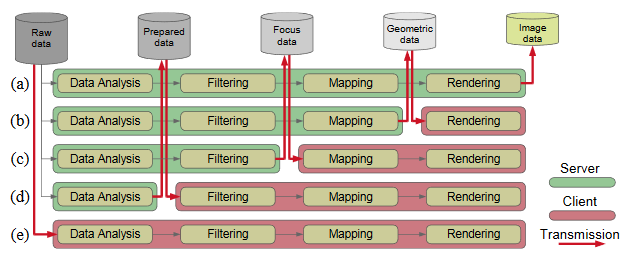
\includegraphics{images/visualization pipeline in client-server scenarios.PNG}
\caption{visualization pipeline in client-server scenarios}
\end{figure}

The raw data is stored on the server, sending the unprocessed data to
the client is a poorly performing approach. The provisioning of large
report files would take too long. Therefore the data need to be
pre-processed on the server. The client should be able to get the
pre-processed, but he can present only a subset of it in each view. One
user scenario is that the analyst takes just a short look at the
dataset. In this case, he sees only one or a few views. Requesting the
complete set of data would result in long initial loading times for each
report. In an improved version the client request only the data the user
wants to see. Therefore the server subsets the data for specific
views.\\
Further work on the server side, like mapping or rendering the data (45)
would speed up the clients loading time enormously (46). But on the same
scale, it would increase the required processing power on the server.
For many clients, this solution would not be scalable. Because of that
option \emph{c} in the figure will be implemented.

The more generic reference model for data visualization by Ben
Shneiderman helps to further distinguish the tasks between server and
client. The server will handle all data, while the client will present
the visual forms. The data transmission between the two components
should be implemented in a standardized way, which allow parameters for
the different views and files. The model distinct also the routing task
between client and server. The server makes the rooting between the
different files/data sources. He will route the client to the reporting
component for this file. The client, on the other hand, will handle the
routing between the different views of the selected dataset.

\section{Backend technology
requirements}\label{backend-technology-requirements}

According to the architecture, the backend has three main tasks: reading
data in different formats, analysis and pre-processing the data and the
provide the data in a standardized way. Additionally, the backend needs
to deliver the web pages to the clients.

The server should provide an application programming interface (API) for
the client. That enables the client to relay on a standardized queries.
The interface should be implemented with a stateless protocol. A
stateless protocol is simple to use and to implement. The simple
protocol makes the testing of the interface easier. A stateful
implementation would perform better a few clients, but with too many
open connections the application would crash. When using stateful
protocol the server would need to keep the large data tables in memory,
and so the application would scale badly. Another advantage is the loose
coupling between client and server, this simplifies independent
development of front- and backend.(47)\\
The most common programming paradigm for stateless web request is the
Representational State Transfer (REST) (49). The REST interface also
improves the scalability of the application. Since each query is
context-free, each query needs the same amount of resources. This makes
it easier to scale the application and identify bottlenecks in the
application. When focusing on the frontend, the REST API will not
restrict the technology or language that can be used. This enables this
work to experiment with different frontend solutions without changing
the backend. It's also helpful for using different types of frameworks
based on the report type.\\
An emerging technology in this area is also GraphQL (50). While GraphQL
is great for performing highly specialized query's. It adds unnecessary
complexity to a simple API service (51). Since the planned API provides
only a subset of the report in a table pattern, without any filter
condition REST will be the better choice in sense of complexity and
maintainability.\\
Together with the web request, the application has to handle normal HTTP
request to deliver the frontend application. For a reliable and fast
user interface these request should be handled by a fast and lightweight
web framework, with REST support.

Reading and analyzing the report data from different formats is the core
backend feature. The backend has to handle the diversity of the
different formats without deduction of performance or extreme
incensement in code complexity. Therefore the backend language should
provide fast I/O operations and libraries that can work on large
datasets. The libraries should be able to import, filter and provide
different kinds of as textual and tabular data. The backend should also
run scripts on the shell, to work with the binary blobs from profiling
tools.

\section{Dashboard technology
requirements}\label{dashboard-technology-requirements}

\subsection{Required frontend components}\label{sec:frontend-req}

The dashboard will be integrated into the existing application for
browsing the performance reports. The users don't need and want another
interface for viewing the reports, building another graphical or web
user interface would be counterproductive. This means the dashboard
development is web-based. A web-based application has also other
advantages for the use case like device diversity or bookmarking of
important views (52).

The web application is based HTML documents which will be styled by CSS
stylesheets. The dashboard reacts to user interactions, routes between
views and needs to visualize structured data. To modify the static HTML
documents, most effort will go into the JavaScript (JS) code, which is
able to manipulate the existing Document Object Model (DOM) of the HTML
files.

To implement the frontend tasks, each task will be supported by at least
one frontend component. The components are simplifying the
implementation by providing different programming interfaces. The
frontend stack contains three components: a framework for building user
interfaces, a kit of style elements and visualization library

The UI framework is required to handle the user interaction to build and
route the different views. The styling components ensure a consistent
user experience and provide building blocks for the UI forms. The
visualization library handles the frontend part of the visualization
pipeline. It will map the data into visual structures and render them.
The following three chapters analyze the requirements for each of these
components based on the use case study.

\subsection{Requirements for the UI frameworks}\label{sec:uilib-req}

The UI library will be chosen based on the following criteria's
separately per report module. The main reason for using such a library
should be to \textbf{improve programming speed}. Therefore a library
should only be chosen, to make the code more readable and add no
unnecessary extra complexity. The library should be lightweight,
flexible and \textbf{easy to integrate} in the current application
stack. As discussed before for the API interface the application and
therefore the frontend should be \textbf{scalable}. Effectively this
should also mean that the library has a \textbf{robust performance}. The
performance should also be testable without an extra application layer.
Finally, the library should be \textbf{stable} and good to trust. This
means it should be widely used or backed by a big company. Since this is
a cooperate work, all libraries have been available under a license
\textbf{free for commercial use}. The support for native development
will not be taken into account. (53)

\subsection{Requirements for styling components}\label{sec:style-req}

On top of the UI library, styling components are necessary. These
improve the building speed and provide a consisted layout. The existing
layout application is based on Bootstrap version 3. Since the UI will be
extended extensively. The requirements for the new report modules are
the determining factor. The existing UI has only one view, changing its
layout can be done without much effort. Independently on the chosen UI
Styling Component, it's must be used in the complete frontend to provide
a consisted User experience (29). Which design language the User
Interface is using is in this state of application not important. The
main User Experience (UX) requirements are reliability, speed, and
flexibility to structure and interact on the interface (38).\\
\\
Therefore styling frameworks with a \textbf{huge number of components}
are required. The dashboard reacts to user input, therefore the
framework needs a large part of form components. The components should
also be \textbf{reactive}, meaning they are designed for user
interaction. Instead of static components, they should be able to handle
their state on their own. This simplifies the development of the
components. On the other hand, the framework should be lightweight, for
a good interaction speed. A \textbf{modular} UI kit can achieve this
balancing act. The framework should implement \textbf{modern features}
like grid breakpoints for Responsive Design and CSS Preprocessor support
for SASS or LESS. (54)

\subsection{Requirements of visualization libraries}\label{sec:viz-req}

While the UI library will handle all user interaction, the actual
visualization of the data has to be done by a charting library. For
these library counts the same as for the UI library, it has to be free
for commercial use. It also should be \textbf{independent of the chosen
framework} or on a huge amount of other libraries. UI-Frameworks have a
short lifecycle (55). This leaves the possibility to switch the
UI-Framework at a further time, without losing all effort brought into
the visualization. In general \textbf{compatibility} with different
UI-Frameworks and devices should be given. To ensure the future
compatibility the library should also be evaluated based on it's
continuous \textbf{enrichment and maintenance over time}. An active
project ensures also the \textbf{documentation} and so the development
effort to be expected. Since the data to be analyzed is huge, the
library should provide the best \textbf{performance} possible, taking a
more complicated implementation into account. It should also
\textbf{support the API format} in which the backend is providing the
data. The main goal of this work is to provide a highly customized
dashboard for the requirements of the Z performance analysts. Therefore
the library should provide a \textbf{wide range of visualization} and as
much \textbf{customization options} as possible to increases the options
in the visualization. (56)

\chapter{Evaluation of the application
technologies}\label{evaluation-of-the-application-technologies}

After deciding on some basic architectural patterns and discussing the
different technology requirements, this chapter can evaluate the actual
technologies for the application stack. Hereafter the one technology
choice in the backend and the three decisions in the frontend will be
under discussion. The backend choice is primarily for the web framework
with some consideration for the language environment. In the frontend
the choice for the UI-framework, the styling components and the
visualisation framework is under evaluation.

\section{Data preparation and backend
technologies}\label{sec:backend-tec}

The existing backend is using a Flask(57) environment on Python for
browsing the server's directories and dynamically render the web pages
with Jinga2(58). This work aims to extend this application. For reasons
of efficiency keeping the existing code basis would be helpful.
Nevertheless if based on programming effort or performance a switch of
programming language and framework would be necessary, this should be
considered. This chapter will discuss benefits of the different possible
web backend's and highlight the best choice for this application. Based
on the choice of programming language the possibilities for data
preparation will be explained.

To handle the web requests the backend requires a web framework.
According to the Web Framework Benchmarks from TechEmpower (59), the
existing Python solution is not the fastest environment around.
Independently of the test-type, languages like Go, Scala, Java or C++
are performing better than the Python frameworks. Additionally to the
normal web requests, the application handles primarily REST calls. These
REST requests require to serialize the analyzed data into JSON. Looking
at the TechEmpower benchmarks, the JSON serialization test runs seem to
match best our utilization scenario. When only looking at request per
seconds data, Java servlets are providing the best results for JSON
Serialization with about 560k queries. The best python library is
providing 87.5\% of the top performance. The best overall results for
plaintext queries are providing C and C++ libraries with about 4 million
queries. Python reaches only 35.3\% of this top score.\\
The switch to Java or C/C++ would require a huge amount of time to set
up the new environment and rewrite the code. Since the application is
not meant to be a high-performance application, the extra amount of time
satisfies not the benefits. A good compromise between performance and a
simple to implement solution could also be Go(73.0\%) if performance
would get more important (60). Another try to improve performance if
it's getting necessary could be to switch to a more performant web
framework of python.

When taking a more specific look at python libraries in the TechEmpower
benchmark. It's quite clear that Flask is not providing the best
performance overall. The best-tested libraries for JSON and Plaintext
queries in mid-2017 seem to be falcon (432k /804k) and wheezy.web (377k
/956k). An older python specific benchmark test shows the same tendency
(61). Both are not including a template engine for server rendering. If
this would be a necessary requirement, if the login mask and the file
browsing component stay in the backend. In this case bottle or weppy are
better alternatives. There are multiple fast and uprising web frameworks
(62) like Sanic or Japronto that have not been covered in the latest
TechEmpower benchmark. The latter promises about 1.2 million plaintext
queries per second (63), which would be even faster than the fastest
frameworks from the TechEmpower benchmarks. But since there are not
comparing in the same benchmark it's hard to compare them equally. Ether
way Flask seems to have only a quarter of the performance that is
possible in the Python environment. For further improvements in
performance, a switch to the falcon or wheezy.web framework should be
considered.

Another important use case for the application is the I/O disk
performance. Reading the data possible into memory is also faster with
compiled languages like C++, Java or Go. These programming languages do
also provide efficient libraries for CSV files, as required by the
sarcsv files. These libraries, like fast-cpp-csv-parser for C++, may be
not as intuitive as the pandas library in Python but even thought fair
enough in terms of usability. But filtering these data sets in C++ would
become then much more complicated in C++. In Java (or Scala) fast
reading and filtering is simpler to implement by using the Apache Spark
framework in local mode, since the programs runs on a single machine.

Even tough no programming language provides such a simple and fast
implementation process for this problem. This point is also the main
reason for staying with Python. The goal of this work is to implement a
working prototype, within a short time frame. The main focus is more on
the a larger feature set, then on high performant application. Since the
performance of the Python environment is fast enough for the current
scale of the application a switch of the programming language is not
required.

Despite the fact that python may not be the fasted language (64) to
solve this problem it has multiple other advantages. Python is an
interpreted language with a simple and readable syntax. According to its
author Guido van Rossum, one of the main concern when developing the
language was \enquote{\emph{to make Python code highly readable}} (65).
This goal has been fulfilled as shown in a comparison based on
expressiveness (66), where Python is ranking significantly better than
most other languages for this use case. Even with the readable language
design, the syntax keeps flexible, when leveraging optional
object-oriented or functional design patterns. Altogether this minifies
the development and debugging time. In terms of efficiency, this is a
huge cost saver and makes the application more fault tolerant. On top of
that python is great in combining different technologies and languages
and provides a comprehensive documenting system with Sphinx (67). (68)

Handling data structures in Python is simple compared to other
programming languages (70). This can be done also in other languages
which are providing even more libraries for different use cases (71).
But Python is providing the most efficient libraries in terms of
documentation and flexibility (72). The main libraries that will be used
in this application will be Pandas and NumPy for reading and modifying
the which is for most of the reports table based. All other work like
the visualization of the data will be done on the front end.

To summarize this chapter, there are good alternatives for the backend
languages or frameworks. But until the performance of our application is
not getting the main concern. The current solution the most efficient
way to solve the given problems and develop the application. For the
project time frame of 7 weeks, this is equally important and therefore
the best tool of choice.

\section{Choose of frontend
technology}\label{choose-of-frontend-technology}

It is no question that JavaScript technology is changing rapidly (73).
Every year a new ECMA specification releases, new JavaScript frameworks
are emerging or getting outdated and together with the frameworks the JS
environment is shifting. This chapter will summarize the state of the
JavaScript environment. How does a common JavaScript application stack
look like in 2018. Which technologies are getting preferred and what are
there competitors. The main focus on the JavaScript technologies, will
be determined by the technologies required in the architecture
sec.~\ref{sec:frontend-req}. In this context the common JavaScript
application context will describe shortly, continued by the evaluation
of UI frameworks and style components for them. The last part in this
chapter will then cover with which visualisation libraries the data can
be visualized.

\subsection{JavaScript development
stack}\label{javascript-development-stack}

The development in JavaScript does not require an extra application
stack. Basically every JavaScript can be embedded directly into a web
page and would be working. Nevertheless all tools in the JS development
stack have been developed on purpose. By understanding this purpose and
there functionality they can simplify the development and even improve
the web performance.

This chapter will introduce six different kinds of tools on which most
JavaScript frameworks are requiring for the development (74).\\
The most important tool in this stack is the package management. The
package manager creates the project structure and installs all project
dependencies. The Node Package Manager (NPM) is the de-facto standard.
It can be configured through the \lstinline!package.json! (75).\\
JavaScript exists in different language flavors. The official JavaScript
is standardized by ECMA(76). Most browsers in the market are only
implementing the ES5 specification. To work with newer versions of the
ECMAScript (ES) or to use other flavors like TypeScript or Elm a
transpiler is necessary. The transpiler converts the syntax into older
versions of ES which are supported by a larger variety of devices. The
most used transpiler in JS is called babel.\\
Like most other programming languages JS has tools for linting and
testing the code. The linter is often used with a task runner, running
while typing the code and detecting bugs or undefined behavior. The most
common linter is ESLint. The tool can be configured with presets like
the airbnb style guide, is then visualizing bad written code segments.\\
To test the JavaScript app one can be chose from many testing suites.
Jest is very popular, but also other frameworks like Jasmine, Mocha or
Tape are commonly used. Jest is very popular because it tests based on
snapshots of the application. So it can test the state changes in the UI
framework and runs test only on the updated components (77).\\
When deploying an JavaScript application the JS files should be minified
to improve the page loading. Also the necessary dependencies should be
loaded linked into the HTML file. A bundling tool, like Webpack
automates this task.\\
It is also possible execute all the previous tools based on some
conditions, like changes in the code. Therefore task runners like Grunt,
Gulp or Broccoli are developed.

\subsection{Dynamically updating the Document Object Model
(DOM)}\label{dynamically-updating-the-document-object-model-dom}

Based on the web statistics by W3Tech (78) jQuery is still the most used
JavaScript library to modify websites. There are also multiple
JavaScript Frameworks, which claim to be the best (55). The main
JavaScript-Framework competitors are React, Angular, and Vue.js.
Indifferent which JS framework will be chosen, it should only be used if
necessary. Using a UI framework will slow down the page loading as more
powerful the framework gets. This means plain or jQuery web pages are
faster than a web pages build by a UI framework (79). Nevertheless
reporting modules with a complex interface, like many subpages or
complex routing between pages, will require a UI-Framework instead of
plain JS.

Therefore the three UI-Frameworks will be evaluated in the further
comparison. Based on web page usage (78), the GitHub stars (80) and the
npm downloads(81) React is beating the other front-end frameworks. But
as seen in (80) Vue.js is growing faster and may become the main
competitor to React (82), whereas Angular has been beaten in this
ranking.

The reason to use the jQuery library instead of plain JS with ECMA5
syntax is that it makes coding faster and easier to understand (83).
Anyway adding the jQuery dependency to use only one feature might not be
reasonable, since there are always plain JS solutions for a jQuery
function (84). This is getting even more enforced, since the latest
specifications of JS EMCA6+ and now upcoming EMCA2018 (76) have an
increased feature set of JS (85). The incompatibility of the newer
specifications with an older browser can be overcome by transpilers like
babel.\\
In large projects, however, UI-Frameworks are handling better the
complex changes of the DOM. Where jQuery sites are requiring many
callbacks and event listener to handle asynchronous code execution,
frameworks are providing an interface to change the state of the page.
The huge amount of references in the plain JS based web pages makes it
harder to understand the code basis.

\subsubsection{Evaluated UI- Frameworks}\label{evaluated-ui--frameworks}

UI frameworks bring new features in the frontend without making the
source code unreadable. The web code written with a framework becomes
usually more modular and structured. This makes the application
components better testable and reusable. The framework makes it possible
to navigate between different subsites, without losing the data model or
loading a new HTML file. Each framework implements these features
slightly different. In the following, they will be described shortly.

React describes itself as \enquote{a declarative, efficient, and
flexible JavaScript library for building user interfaces} (86). The
first version was released in 2013, now 16.2.0 (87) is the current
version of the library maintained by Facebook. The main characteristic
of the library is the reactive approach. This approach means if the
state of a component changes React is automatically rerendering the
Virtual DOM (88), by using its reconciliation algorithm (89). The
Virtual DOM is a virtual representation of the browser views in the
memory. Applications written in React are divided by their functionality
into components. This means JavaScript is generating the HTML by
defining both business logic and HTML markup (90). React used therefore
a syntax extension called JSX. Furthermore React is only a core library,
it's used in general together with React-Dom for the Virtual DOM in the
browser and several other extensions. (91)

Whereas React is backed by Facebook, Google is behind the development of
Angular. The first version of Angular (AngularJS) was released in
October 2010. A complete has then been done into Angular2 (September
2016), on which all newer Angular Versions are based on. The current
version is 5.0.1. In contrast to its competitors, Angular relies on
TypeScript. TypeScript is an extension of JavaScript based on the
suggestions for EMCA6 developed by Microsoft (92). The main features
static typing and improvements for object orient concepts (93).\\
Angular has also a strict separation of technology and components. In
contrast to React TypeScript is used to extend the HTML by creating HTML
\emph{templates} with Angularized markup. These templates are managed by
\emph{component} classes and the actual application logic is inside the
\emph{services}. Together they are boxed in \emph{modules}. Every
Angular App has a \emph{bootstrapping} the \emph{root module}, from
where on Angular takes over the navigation, presentation and user
interaction. This separation of different components follows strictly
the model-view-controller pattern. Additionally Angular is providing
most functions in its core dependencies and almost predefined workflow
for the development. (94)

Vue.js is the youngest of the three frameworks, introducing it's the
first version in February 2014 and the current version 2 in 2016. It's
not developed by a big company, instead of by a small team of a dozen
developers led by Evan You. Even though large companies like Alibaba or
Baidu are using it. Vue.js has borrowed most of its concepts from its
successors like Angular, react or Ember.js. Like React Vue.js utilizes a
virtual DOM and provide reactive and composable view components. But
addition it integrates frequently used features like routing and global
state management in the core library. In contrast to Angular or React it
forces the user not to learn superset of JavaScript, like JSX or
TypeScript. The top priority of Vue.js is to provide a lightweight and
easy to learn library for user views. (95)

\subsubsection{Comparison of the UI
frameworks}\label{comparison-of-the-ui-frameworks}

All three libraries have their eligibility for different domains, the
evaluation will choose the best match based on the criteria defined in
the chapter before. All libraries are using the MIT license, so the k.o.
criteria of being used without any license cost are fulfilled. (96)

In terms of programming speed, Vue.js is the best framework. According
to several articles, it has the fastest learning curve, together with a
very simple syntax that requires no extra technology like JSX or
TypeScript. Not so easy to learn but also fast is React since it is only
a simple JS library to implement with great flexibility in the workflow.
Angular has a harder learning curve since it's very complex, but
TypeScript (which is also available for React) improves the readability
of the code. In large projects, the scalability of the development time
is better with more developers (98). All libraries are providing a solid
documentation to learn the framework.

In point of integration into the application environment, React and
Vue.js are equally straightforward. The reason behind this is, that both
are only JS libraries, which can easily be imported in normal JS files
without the need extra build dependencies like angular is requiring it.

The scalability can only be rated by way of deploying an application.
Angular brings its strengths in large Single Page Applications (SPA)
because it was built for them (99). Because of the strong enforcement
for modularity, large projects are better maintainable and suitable for
larger pools of developers. Angular is also easily testable and
therefore better scalable. React and Vue.js can more easily be used for
microservices since they require only simple imports of JS libraries.
This enables better scaling for large environments. React is even better
for microservices since every functional component of React is a single
module. Because of the huge amount of libraries React is also better for
complex projects.

As shown in the js-framework-benchmark the frameworks cannot compete
with the fastest framework available. There compared performance is
almost one level. Vue.js is slightly faster, but the benchmark from
mid-2017 is also not using the newest versions aka React 16 and Angular
5. Especially in React 16 with React Fiber (100) has made huge
performance improvements under the surface. Important for the speed of
the initial page loading, can also be the library size. Since Vue.js is
the most lightweight it is in general faster, whereas Angular is the
slowest one.

React and Angular have the backing of two of the most powerful
companies, in financial aspects as well as in their skill in the area.
Vue.js, on the other hand, is founded via Patreon even tough it get used
by Baidu and Alibaba. Based on the npm downloads React is definitely the
most used framework of them three. React is also the most popular one
based on the stateofjs survey (101) and the GitHub stars (80). Even
though the community of Vue.js is growing faster at the moment.

React is the winner for this comparison based on the huge environment
supporting it and it's high popularity. The workflow of React is very
flexible so that it is easily integrated into the current application
environment. Vue.js stands out with a simple and lightweight framework,
which would make development, even more, easier than React. Even though
its only one of many uprising technologies. Vue.js may success React
(82), but at the moment React is a safer choice of tool. React is backed
by a big company and the most popular framework for now. The framework
very simple to implement and fulfills the necessary requirements.
Together these points make React the best choice as the framework for
the more complex multipage sites.

\subsection{Styling the User
Interface}\label{styling-the-user-interface}

The decision on the styling components has no huge effect on the
application. The styling components can be changed easily changed and
aesthetics are a matter of taste. The main requirements for the styling
components are that they can be used with different UI-Frameworks. The
support of different UI-Frameworks makes it easier to substitute the
underlying UI-Framework layer. The small reports may also only use
jQuery or even no library.

If IBM provides a suitable framework for the application this would be
the most consistent style component choice. At the moment internal
design framework for the internal w3 design is not publicly available.
IBM provides only the Carbon Framework (102) used by IBM Cloud. This
framework has not been chosen, because it provides not enough form
components for the user interaction. According to the GitHub statistics
Bootstrap, Semantic-UI, Foundation, Materialize and Material UI are the
five most popular UI-Frameworks. The frameworks have an equal features
set in most categories. All are licensed under MIT. Some frameworks are
more modular and performant than other, but the differences are to
slight to make a significant distinction. All styling components have a
responsive design and can be used together with CSS preprocessors.\\
The frameworks are suitable for complex user interactions, with
exception of the Foundation framework. This framework has not enough
form elements for the required filtering components.\\
\\
For the Material Design framework, Bootstrap and the Semantic UI
components exist implementation for all discussed UI-frameworks.\\
This makes the choice of the framework and aesthetic choice. I like the
Material Design by Google the most. Because of that I choose the
Material-UI for the React Framework and Materialize for jQuery. (103)

\subsection{Visualizing the data}\label{visualizing-the-data}

This chapter evaluates the libraries for the core feature of this work,
the visualisation. Since there is a huge amount of options this chapter
will firstly filter the visualisation libraries before comparing them on
the given criteria's.

\subsubsection{Filtering visualization
libraries}\label{filtering-visualization-libraries}

Despite the user interactions on the dashboard, the data visualization
is the main focus of the dashboard. For efficiently creating a huge an
amount of plots for different views and datasets the use of a library
cannot be avoided. There many visualization libraries for JS. To get a
glue of the numbers, GitHub is listing about 850 JavaScript projects
(07.02.2018) under the term visualization (105). This chapter can focus
only on a subset of the available libraries. Since this work relies on
some mandatory requirements, libraries which not match the following
criteria will not be considered. The library must be open source and
\textbf{free for commercial use}. This disallows libraries like
Highcharts, FusionCharts, and ZingChart. Since the analyzed data is
confidential, the visualization has to be done \textbf{locally} without
leaving the Intranet. This prohibits API solutions like Google Charts
even if there are free or commercial use. To leave the possibility open
to switching the UI framework, the visualization library should not be
\textbf{depended on frameworks} ones like Ember Charts, Victory,
ReCharts or jqPlot. The reports are requiring a huge amount of different
charts which should ideally implement with only one library unless there
is a special use case which requires a special library. Therefore
specialized libraries like Timesheet.js, VivaGraph, Sigma.js, Leaflet or
heatmap.js are unsuitable. Only charting libraries are considered.

The focus report of this report is not a complete comparison of all JS
charting libraries. Only the most important libraries will be evaluated.
The distinction is done by GitHub star ranking and npm download
statistics. Only projects with over 1k stars and npm downloads per day
will be considered. This condition limits the list to D3.js, Chart.js,
C3, Raphael, NVD3, Chartist, ECharts, plotly.js, Vega, Vega-Lite and
Vis.js (106). In both rankings, D3.js and Chart.js are completely
outstanding. D3 is complete outstanding by even doubling both numbers of
Chart.js. In the further course of the chapter, the 10 different
libraries will be shortly introduced with there main features and then
compared based on the criteria defined in chapter
sec.~\ref{sec:usecase-result}.

\subsubsection{Introduction of possible visualization
libraries}\label{introduction-of-possible-visualization-libraries}

The most popular library for data visualization is D3.js (107) also
known as D3 or Data Driven Documents. The library is based on Protovis
and has 2 actively maintained versions v3 and v4. This evaluation will
refer to the newer (and better) version (108). One of the reasons for
the popularity is the flexibility of D3 (109). It is able to manipulate
the DOM and integrates the existing web technologies, like Scalable
Vector Graphics (SVG) and Canvas to create the visualizations. The
library can be used for any visualization project, because of it's BSD
3-Clause, which allows commercial use as well. Using D3 for different
projects becomes even easier since D3 has a comprehensive API
documentation (110) and an own platform for example visualizations with
Bl.ocks (111). If some kind of visualization not supported there is a
high change a plugin to solve this is already written, This list is
proving an overview about the D3 plugins \cite{awesome-d3}. The
visualization by D3 itself is fast and D3 can handle huge amounts of
data compared to other libraries. The actual speed of the rendering
performance depends on the underlying technology. Canvas is much faster
the SVG graphics as shown in this performance benchmark (112).

Many visualization libraries are using d3 and abstracting its complexity
and low-level interface to an easier to use interface. From the current
selection C3, NVD3, plotly.js, Vega and Vega-Lite are based on D3. Each
of the four libraries has different levels of abstraction (113).\\
NVD3.js has the highest level of abstraction of the four. The library is
developed by Novus Partners and distributed with the Apache 2.0 license.
The syntax is close to the original d3 library but only rudimental
documented and with a few possibilities. The library supports also only
the basic types of diagrams: bar, bullet, line and pie charts. Each of
the charts is provisioned with animations.\\
C3 indifference has a more extensive visualization API. The library is
developed since 2013 by Masayuki Tanaka under MIT license. The
visualization for C3 is done by a model definition in JSON. Compared to
NVD3 it has less visual effects. The API parameter, on the other hand,
is highly customizable and well documented. In contrast to NVD3, there
is also no more coding in d3 required. This makes it a lot easier to use
but, looses also the customization possibilities of d3.\\
Another D3 based library is called plotly.js. It's the JavaScript
implementation of the declarative Plotly API. The visualization
description exists for Python, Matlab, and R and is developed and
distributed by the Plotly Inc. under MIT license.The framework is built
on top of d3.js and stack.gl and provides over 20 different chart types.
The documentation side provides an extensive API description together
with many examples.

Like C3 or plotly.js, Vega (114) and Vega-Lite (115) are also
declarative visualization languages based on a JSON syntax. The
languages are build by the Stanford Visualization Group, now called the
University of Washington Interactive Data Lab. The same group that
developed D3. Vega is not intended as a replacement for D3 (116). Like
D3 there are both licensed under the BSD-3 clause. D3 is meant to be a
low-level visualization framework, whereas Vega provides an abstract
layer for representing and reasoning visualizations. The idea behind the
project is to \enquote{promote an ecosystem of usable and interoperable
tools, supporting use cases ranging from exploratory data analysis to
effective communication via custom visualization design}. The
abstraction layer has also various improvements for Browser
compatibility since there are translated in runtime to D3 code based on
the environment. Vega-Lite is based on Vega and provides a higher level
grammar to enable fast specification of interactive data visualizations.
Both libraries provide an enormous amount of different charts and a very
extensive documentation.

The main competitor of D3 according to usage stats is Chart.js. Like C3
or Vega, the charts are described with a JSON Model. The library
supports 8 highly customizable chart types, which cover almost all use
cases. Chart.js provides multiple examples for these charts and the API
is well documented. Chart.js is actively maintained by seven different
developers and published as Open Source with an MIT license. Chart.js
has good plotting performance using HTML5 Canvas. It also supports
responsive rerendering. Like D3 it also can be extended by plugins.

Raphael is a lightweight library for drawing vector graphics. It is
developed by Dmitry Baranovskiy under MIT license. In contrast to the
other libraries, it's the oldest release is a bit older than a year. The
library is easy to use for visualizations, but it is not scoped for
charts. This makes plotting charts harder to implement than in D3.
Especially for older devices or a great compatibility Raphael is a good
choice because of its unique support of the Vector Markup Language
(VML), SVG and Canvas objects.

Chartist is a lightweight charting library for customizable responsive
charts. Gion Kunz is the main developer of the library and licensed it
under MIT. Chartist can create three different kinds of plots bar, pie
and line charts. There are plotted into SVG and can be animated with the
Synchronized Multimedia Integration Language (SMIL). To implement the
charts, Chartist.js provides detailed examples and an API documentation.
Chartist is also extendable by plugins.

The vis.js visualization library (117) initially developed by Almende
B.V. and dual licensed under both Apache 2.0 and MIT. The library
designed to be easily usable and to handle large amounts of dynamic
data. The library consists of five main components: DataSet, Graph2d,
Graph3d, Network, Timeline. For the use case important is the Graph2d
component which plots data into bar or line charts. Pie charts are not
possible which makes the library unsuitable for the visualizations
purpose.

ECharts is a powerful charting library developed and maintained by
Baidu. ECharts provides a large number of possible visualizations in two
and three dimensional. The library is based on zrender, which uses
Canvas for the plotting, but ECharts is also available as a WebGL
version. It can also be integrated with several UI Frameworks or GIS
applications and has implementations in many other programming
languages. The JavaScript implementation is licensed under BSD 3-Clause.
The website provides many complex visualization implementations. The API
is documented in English and Chinese, even though the main language in
almost all user forums is Chinese.

\subsubsection{Decision on the best charting
library}\label{decision-on-the-best-charting-library}

The previous chapter has given a short overview of the most popular
JavaScript visualization libraries. This has only a small subset fitting
for the visualization requirements. The decision on the visualization
depends mainly on the balancing between simplicity and performance of
the implementation. If simplicity is more important Vega or even
Vega-Lite would be a considerable choice. If performance and maximal
customization are important D3 is the best choice. In the following, the
decision on D3 will be explained on the established criteria.

The library should be compatible with a wide range of devices. All
libraries provide a robust compatibility. The high-level frameworks,
like Vega, are abstracting compatibilities between browsers
automatically, so they are a bit better in terms of compatibility. The
best compatibility has Raphael. This is based on the support for old
browsers by VML.\\
The chart implementation with Raphael requires a very low-level
programming of the graphic because the library is not developed for
plotting charts. Libraries like D3 are there more effective in terms of
simple implementation. Vega-Lite is providing here the best compromise
between implantation speed and features.\\
Nevertheless, a big feature set can only be reached with a complex
low-level visualization framework. Besides the performance, this is the
most important feature. The libraries that provide the biggest feature
set are D3 and ECharts. ECharts has the problem that the support is only
available in the Chinese language, whereas D3 has a larger English
community. The D3 community provides example implementations for almost
any use case. D3 is also highly customizable and provides almost any
kind of chart either natively or with a plugin. Additionally, it has a
great performance for a huge amount of data, which makes D3 the best
choice. (118)

\subsubsection{Rendering Graphviz files}\label{rendering-graphviz-files}

In addition to the charting libraries which are dynamically creating
data-driven visualizations, the graph reports will require a simple and
fast rendering library for graphviz files. Graphviz is a old and for the
web very uncommon graph format. There exists a few libraries that port
the graphviz format into the web: livizjs, graphviz.js, graphlibDot and
viz.js. Only two of them are still maintained: graphlibDot or viz.js.\\
graphlibDot has been written from scratch in JS, where as viz.js is
build on the original graphviz source by using emscripten. emscripten is
a toolchain for converting c and c++ in WebAssembly. WebAssembly (WA) is
an low-level assembly-like language than can run in the browser with
almost native performance. If WebAssembly is not supported asm.js is
used. asm.js is not as fast as WA, but also highly optimized (120). This
makes the viz.js library much faster than graphlibDot.\\
Both libraries are not providing an extra features for parsing dot
files. Actually there are no existing JS libraries for parsing the
graphviz files. This makes viz.js the best choice even if it can only
render the dot files.\\
The parsing will be implemented to be manually in the frontend.

\chapter{Implementation of the
Dashboard}\label{implementation-of-the-dashboard}

This chapter will present an implementation overview based on the
architecture and technology decisions presented before. In the first
part, the architecture will be explained in detail. The second part will
present the key implementations of back and frontend. The implementation
samples for the frontend will cover the REST API and the data
pre-processing. The samples for the frontend will include the graph
plotting with D3, the visualization of graphviz files and the page
routing with React.

\section{Dashboard architecture}\label{dashboard-architecture}

The application is designed with a two-tier client-server architecture
(43). The advantage of this implementation that the two layers are
strictly separated and can be developed independently. The layers are
solely communicating over the REST interface. The following graphic
presents the components of the architecture. The Web Layer contains the
complete frontend logic separately provisioned into different report
modules show as 📄 elements. The Python backend handles all web request
from clients which are requesting the report modules. In also handles
the REST requests from the report modules working at the client. In the
following chapters explain the internal structure of the layers as well
as their logic and execution flow.

\begin{figure}
\centering

\includegraphics{C:/Users/PaulBauriegel/Box Sync/DHBW Mannheim/PA5/images/Architecture.png}
\caption{Dashboard Architecture Overview}
\end{figure}

\subsection{Application Frontend - Web
Layer}\label{application-frontend---web-layer}

The frontend environment of the application is a mixture of frameworks
to build the application, the report modules itself and the tools to
deploy the modules. The current solution has four reporting modules for
the four kind of files described in chapter
sec.~\ref{sec:usecase-data}.\\
Each reporting module is a single page app, that contains his own
application stack. The application stack contains the three core
libraries for UI, style and visualisation together with the deployment
tools. All modules share the same basic deployment tools. NPM scripts
for automatic building, the ESLint linter and webpack for bundling and
minifying the JS code. The React based applications are including also
other tools created by the create-react-app boilerplate. The React stack
contains also the Jest testing tool and the babel transpiler.

Each report includes a different combination of core libraries. The
Graph report is visualizing the profiling data. The report is static. It
request only the dot file from the server an makes some basic
manipulation on them like shrinking the function signatures. The viz.js
libraries is rendering these dot files. The other two core libraries
come from the minimized stack. The log-file report are implementing the
same core libraries, but it has a more sophisticated visualisation of
the data. Therefore the D3.js library is used. The sysstat report
implements complex visualizations as well but has also multiple views.
The rendering and routing between of multiple pages is faster when
handles by the UI framework. To accomplish these task React is used in
the backend. The CPI report has the same complexity and used React
therefore. In contrast to sysstat the CPI data report is not visualizing
the data with plots. It's only presenting them in tables.

The minimized stack is handling the REST request with the
\lstinline!XMLHttpRequest!. The react stack uses \lstinline!axios! for
the JSON queries. If the D3.js library is imported the report is using
\lstinline!d3.json! implementation directly.

\subsection{Application Backend}\label{application-backend}

As discussed in chapter sec.~\ref{sec:backend-tech} the backend is
written in Python 3.6. The project has several dependencies.\\
All web request is handled by Flask, the REST interface as well as the
backend rendering and the provision of the web pages. For each report
module the web provisioning has to be extended with the new routing
rules and the data-processing functions. Each report view needs also one
or more REST requests. Each REST Call is bind to the processing
functions.\\
Since each report has different file types and requirements a common
layer is not possible therefore. the only common layer is the data
access, which contains only a few functions.\\
The data preparation has many different tasks. Some performance reports
like the sysstat or the CPI data do contain multiple datasets. The
\enquote{header functions} are iterating over these files to find the
line range of the datasets. The client can request these datasets
separately. Since the backend is RESTful each request will execute an
independent data preparation function. If the data-set is tabular, the
pandas library will handle the call. Otherwise custom log analyzer
functions are processing the request. The pandas library will only load
the requested file-part into memory to transform or filter the dataset
for the client's demands. The log functions are working in a similar
way.\\
The handling of profiling data is an exception to the described RESTful
workflow. Profiling data, e.g.~perf data files, is most cases binary
data and cannot be analyses directly. At first the data has to be
processed by the profiling tool itself. Like in this example for perf:
\lstinline!perf script | c++filt | gprof2dot.py -f perf > perf.data.dot!.\\
Therefore the backend will execute a bash sub-process. After the
serialization by the profiling tool the output is directly piped into
gprof2dot. Gprof2Dot is written José Fonseca and creates a graphviz file
with the corresponding call graph. This dot file is then delivered to to
client.

\section{Dashboard Implementation}\label{dashboard-implementation}

The second part will present the key implementation in the back and
frontend. The implementation samples for the frontend will cover the
REST API and the data pre-processing. The samples for the frontend will
cover the graph plotting with D3, the visualization of graphviz files
and the page routing with React.\\

\subsection{Implementation of the backend
engine}\label{implementation-of-the-backend-engine}

\subsubsection{Data preprocessing in Python
3}\label{data-preprocessing-in-python-3}

\subsubsection{REST implementation with
Flask}\label{rest-implementation-with-flask}

\subsection{Implementation of visualization and user
interface}\label{implementation-of-visualization-and-user-interface}

\subsubsection{Page routing with React
v16}\label{page-routing-with-react-v16}

\subsubsection{Visualisation of Graphviz
files}\label{visualisation-of-graphviz-files}

\subsubsection{Data plotting with D3.js
v4}\label{data-plotting-with-d3.js-v4}

\chapter{Conclusions and future work}\label{conclusions-and-future-work}

::: What have been the requirements ::::::\\
Time\\
::: Architeture conclusion ::::::\\
Client Server Application

::: Technology conclusion ::::::\\
Best web framework = Flask because is already used -\textgreater{}
consider switching the web framework in python to wheezy or falcon\\
speak about Python vs.~Go\ldots{}???\\
Best UI-Framework -\textgreater{} react, vue may be a competitor\\
CSS Styling not important\\
Best Visualisation Framework -\textgreater{} D3

::: Implementation conclusion ::::::\\
- four reports, with difernet coverage and aspects -\textgreater{}
further work have to be done -\textgreater{} more reports, more plots
-\textgreater{} \ldots{}

::: Further Work ::::::

live stream data, while the report is running

single sign-on IBM

interconnect the reports

plugin structure

::::::::::::::::::

\chapter*{Literature}\label{bibliography}
\addcontentsline{toc}{chapter}{Literature}

\hypertarget{refs}{}
\hypertarget{ref-Hottelet.2017}{}
1. HOTTELET, Ulrich. \emph{Der bilanzierte kunde: Der wert von daten für
die digitalökonomie} {[}online{]}. 2017. Berlin.
{[}Accessed~6~February~2018{]}. Available from:
\url{http://businessimpact.eu/der-bilanzierte-kunde/}Sie gelten als
Schmierstoff der Digitalökonomie und ihr Wert steigt und steigt:
(Kunden-)Daten sind das Öl des 21. Jahrhunderts.

\hypertarget{ref-Wongsuphasawat.2016}{}
2. WONGSUPHASAWAT, Kanit, MORITZ, Dominik, ANAND, Anushka, MACKINLAY,
Jock, HOWE, Bill and HEER, Jeffrey. Voyager: Exploratory analysis via
faceted browsing of visualization recommendations. \emph{IEEE Trans.
Visualization \& Comp. Graphics (Proc. InfoVis)} {[}online{]}. 2016.
Available from: \url{http://idl.cs.washington.edu/papers/voyager}

\hypertarget{ref-McIntosh.2013}{}
3. MCINTOSH, Colin (ed.). \emph{Cambridge advanced learner's dictionary}
{[}online{]}. 4. ed. Cambridge~: Cambridge Univ. Press, 2013.
ISBN~9781107035157. Available from:
\url{https://dictionary.cambridge.org/dictionary/english/visualize}

\hypertarget{ref-Earnshaw.1992}{}
4. BRODIE, Ken W., LA CARPENTER, EARNSHAW, R. A., GALLOP, HUBBOLD, R.
J., AM MUMFORD, OSLAND, C. D. and QUARENDON, P. Scientific
visualization. \emph{Scientific Visualization: Techniques and
Applications}. 1992. P.~1--3.

\hypertarget{ref-Owen.1999}{}
5. OWEN, G. Scott. \emph{Definitions and rationale for visualization}
{[}online{]}. 1999. {[}Accessed~10~February~2018{]}. Available from:
\url{http://www.siggraph.org/education/materials/HyperVis/visgoals/visgoal2.htm}

\hypertarget{ref-Senay.1994}{}
6. SENAY, H. and IGNATIUS, E. A knowledge-based system for visualization
design. \emph{IEEE Computer Graphics and Applications}. 1994. Vol.~14,
no.~6, p.~36--47.
DOI~\href{https://doi.org/10.1109/38.329093}{10.1109/38.329093}.

\hypertarget{ref-Posada.2017}{}
7. POSADA, Juan Carlos Morales. On the meaning of data visualization,
information visualizationand information graphics.
\emph{meta-carto-semiotics} {[}online{]}. 2017. Vol.~8, no.~1, p.~1--13.
Available from:
\url{http://ojs.meta-carto-semiotics.org/index.php/mcs/article/view/9}During
each investigation process, the number of terms used to define the
subject matter in question is directly proportional to the number of
analytical perspectives taken on this subject. This phenomenon is both
normal and symptomatic for the different processes of knowledge
generation and re-generation, and can be even considered to be
plausible. However, it is also symptomatic to find terms, which rather
tend to distort the concepts, notions or phenomena they want to refer
to. This is especially delicate when is about to define and delimitate
an epistemological or academic field of research, or when the results of
those investigations need to be published. This paper aims, in the light
of the ethics of terminology by Charles S. Peirce (1998), to analyse
the concepts information design, data visualization, information
visualization and information graphics regarding possible terminological
distortions. Moreover we shall discuss, if such distortions can hamper
research on the topics mentioned. (This article results from the
author's master thesis in Communicational Design at the University of
Buenos Aires.)

\hypertarget{ref-Gershon.1997}{}
8. GERSHON, N. and EICK, S. G. Information visualization. \emph{IEEE
Computer Graphics and Applications}. 1997. Vol.~17, no.~4, p.~29--31.
DOI~\href{https://doi.org/10.1109/MCG.1997.595265}{10.1109/MCG.1997.595265}.

\hypertarget{ref-Krypczyk.2014}{}
9. KRYPCZYK, Veikko. \emph{Theorie und praxis der datenvisualisierung
\textbar{} entwickler.de} {[}online{]}. 2014.
{[}Accessed~10~February~2018{]}. Available from:
\url{https://entwickler.de/online/datenbanken/datenvisualisierung-theorie-und-praxis-114322.html}Es
existieren die unterschiedlichsten Diagrammarten. Wir führen in das
Thema ein und erläutern die unterschiedlichen Arten von Diagrammen.

\hypertarget{ref-Dassler.1999}{}
10. DÄßLER, Rolf. Informationsvisualisierung: Stand, kritik und
perspektiven. In~: \emph{Methoden/strategien der visualisierung in
medien, wissenschaft und kunst} {[}online{]}. Wissenschaftlicher Verlag
Trier, 1999. Available from:
\url{http://fiz1.fh-potsdam.de/volltext/fhpotsdam/03021.pdf}

\hypertarget{ref-Ackoff.1989}{}
11. ACKOFF, Russell L. From data to wisdom. \emph{Journal of applied
systems analysis} {[}online{]}. 1989. Vol.~16, p.~3--9.
{[}Accessed~11~February~2018{]}. Available from:
\url{http://faculty.ung.edu/kmelton/documents/datawisdom.pdf}

\hypertarget{ref-Chen.2009}{}
12. CHEN, Min, EBERT, David, HAGEN, Hans, LARAMEE, Robert S., VAN LIERE,
Robert, MA, Kwan-Liu, RIBARSKY, William, SCHEUERMANN, Gerik and SILVER,
Deborah. Data, information, and knowledge in visualization. \emph{IEEE
Computer Graphics and Applications}. 2009. Vol.~29, no.~1, p.~12--19.
DOI~\href{https://doi.org/10.1109/MCG.2009.6}{10.1109/MCG.2009.6}.

\hypertarget{ref-Shneiderman.1999}{}
13. CARD, Stuart K., MACKINLAY, Jock D. and SHNEIDERMAN, Ben (eds.).
\emph{Readings in information visualization: Using vision to think}
{[}online{]}. San Francisco, Calif.~: Morgan Kaufmann, 1999. The morgan
kaufmann series in interactive technologies. ISBN~1558605339. Available
from: \url{http://www.loc.gov/catdir/description/els033/98053660.html}

\hypertarget{ref-Chi.Jan.2000}{}
14. CHI, Ed Huai-Hsin. A taxonomy of visualization techniques using the
data state reference model. In~: \emph{Information visualization
(infovis 2000)}. s.l.; Los Alamitos~: I E E E Imprint, January 2000.
p.~69--75. ISBN~0-7695-0804-9.

\hypertarget{ref-DosSantos.2004}{}
15. DOS SANTOS, Selan Rodrigues. \emph{A framework for the visualization
of multidimensional and multivariate data}. PhD thesis. University of
Leeds, 2004.

\hypertarget{ref-Tufte.2001}{}
16. TUFTE, Edward R. \emph{The visual display of quantitative
information}. 2. ed., 1. print. Cheshire, Conn~: Graphics Press, 2001.
ISBN~0961392142.

\hypertarget{ref-Hamed.2013}{}
17. HAMED, Zach. \emph{What makes a good visualization?} {[}online{]}.
2013. {[}Accessed~11~February~2018{]}. Available from:
\url{https://medium.com/@zmh/what-makes-a-good-visualization-d94e8005e530}My
summer at Jawbone and the art of the visualization.

\hypertarget{ref-Abela.2006}{}
18. ABELA, Andrew. Chart suggestions---A th ought-starter. {[}online{]}.
2006. {[}Accessed~12~February~2018{]}. Available from:
\url{http://extremepresentation.typepad.com/files/choosing-a-good-chart-09.pdf}

\hypertarget{ref-Roam.2008}{}
19. ROAM, Dan. The visual thinking codex. {[}online{]}. 2008.
{[}Accessed~12~February~2018{]}. Available from:
\url{http://www.blogtrw.com/wp-content/uploads/The-visual-thinking-codex.pdf}

\hypertarget{ref-Roam.2008b}{}
20. ROAM, Dan. The s.Q.V.I.D. a practical tool of applied imagination..
2008.

\hypertarget{ref-Few.2006}{}
21. FEW, Stephen. \emph{Recommendations for your data visualization
bookshelf} {[}online{]}. 2006. {[}Accessed~12~February~2018{]}.
Available from:
\url{http://www.perceptualedge.com/articles/b-eye/data_visualization_bookshelf.pdf}

\hypertarget{ref-PerceptualEdge.2018}{}
22. PERCEPTUAL EDGE (ed.). \emph{Perceptual edge - library}
{[}online{]}. 2018. {[}Accessed~12~February~2018{]}. Available from:
\url{http://www.perceptualedge.com/library.php}

\hypertarget{ref-Arora.2018}{}
23. ARORA, Harshita. \emph{What's the difference between ux and ui
design?} {[}online{]}. 2018. {[}Accessed~12~February~2018{]}. Available
from:
\url{https://medium.freecodecamp.org/whats-the-difference-between-ux-and-ui-design-2ca8d107de14}And
some tips for you to get started with both.

\hypertarget{ref-Saidy.2017}{}
24. SAIDY, Nicole. \emph{7 steps to become a ui/ux designer -- nicoles
blog} {[}online{]}. 2017. {[}Accessed~11~February~2018{]}. Available
from:
\url{https://blog.nicolesaidy.com/7-steps-to-become-a-ui-ux-designer-8beed7639a95}Tips
\& resources to help you get started

\hypertarget{ref-Farley.2009}{}
25. FARLEY, Jennifer. \emph{Principles of design: Color} {[}online{]}.
2009. {[}Accessed~11~February~2018{]}. Available from:
\url{https://www.sitepoint.com/principles-of-design-colour/}In the final
part of her series on design principles, Jennifer takes a look at the
type of color schemes you can put together to create mood.

\hypertarget{ref-Farley.2009b}{}
26. FARLEY, Jennifer. \emph{Principles of good design: Balance}
{[}online{]}. 2009. {[}Accessed~11~February~2018{]}. Available from:
\url{https://www.sitepoint.com/principles-of-good-design-balance/}Jennifer
describes how balance is important to achieve attractive results in
design.

\hypertarget{ref-Farley.2009c}{}
27. FARLEY, Jennifer. \emph{Principles of design: Contrast}
{[}online{]}. 2009. {[}Accessed~11~February~2018{]}. Available from:
\url{https://www.sitepoint.com/principles-of-design-contrast/}In the
third part of the series on Principles of Design, Jennifer takes a look
at how contrast helps to create eye-catching designs.

\hypertarget{ref-Cronin.2009}{}
28. CRONIN, Matt. \emph{10 principles of readability and web typography}
{[}online{]}. 2009. {[}Accessed~11~February~2018{]}. Available from:
\url{https://www.smashingmagazine.com/2009/03/10-principles-for-readable-web-typography/}**Readability**
is one of the more important aspects of Web design usability. Readable
text affects how users process the information in the content. Poor
readability scares readers away from the content. On the other hand,
done correctly, readability allows users to efficiently read and take in
the information in the text. You want users to be able to read your
content and absorb it easily.

\hypertarget{ref-Nikolov.2017}{}
29. NIKOLOV, Anton. \emph{Design principle: Consistency} {[}online{]}.
2017. {[}Accessed~9~February~2018{]}. Available from:
\url{https://uxdesign.cc/design-principle-consistency-6b0cf7e7339f}The
most known and the most fragile design principle.

\hypertarget{ref-Chesnut.2014}{}
30. CHESNUT, Donald and NICHOLS, Kevin. \emph{UX for dummies}.
Online-Ausg. West Sussex, England~: John Wiley \& Sons, 2014. --For
dummies. ISBN~1118852788.

\hypertarget{ref-Allabarton.2016}{}
31. ALLABARTON, Rosie. \emph{The ux design process: An actionable guide
to your first job in ux} {[}online{]}. 2016.
{[}Accessed~12~February~2018{]}. Available from:
\url{https://careerfoundry.com/en/blog/ux-design/the-ux-design-process-an-actionable-guide-to-your-first-job-in-ux/}What
does a UX designer do day-to-day? Get an in-depth introduction to User
Experience (UX) Design processes.

\hypertarget{ref-Lam.2016}{}
32. LAM, Thai. \emph{6 steps in a common ux design process}
{[}online{]}. 2016. {[}Accessed~12~February~2018{]}. Available from:
\url{https://blog.prototypr.io/a-common-product-ux-design-process-55af4ab5665e}I
got many questions from my friends. So what design process do I use? How
do you start? What and how many steps are there? If I just say\(\ldots\)

\hypertarget{ref-Nunnally.2017}{}
33. NUNNALLY, Brad and FARKAS, David. \emph{UX research: Practical
techniques for designing better products}. Beijing~: O'Reilly Media,
2017. ISBN~1491951249.

\hypertarget{ref-Levy.2015}{}
34. LEVY, Jaime and CALACANIS, Jason. \emph{UX strategy: How to devise
innovative digital products that people want}. First edition.
Sebastopol, CA~: O'Reilly Media, Inc, 2015. ISBN~9781449372866.

\hypertarget{ref-Goltz.2014}{}
35. GOLTZ, Shlomo. \emph{A closer look at personas: What they are and
how they work \textbar{} 1} {[}online{]}. 2014.
{[}Accessed~12~February~2018{]}. Available from:
\url{https://www.smashingmagazine.com/2014/08/a-closer-look-at-personas-part-1/}

\hypertarget{ref-Ambler.2014}{}
36. AMBLER, Scott W. \emph{User stories: An agile introduction}
{[}online{]}. 2014. {[}Accessed~12~February~2018{]}. Available from:
\url{http://www.agilemodeling.com/artifacts/userStory.htm}

\hypertarget{ref-Turner.2010}{}
37. TURNER, Neil. \emph{A step by step guide to scenario mapping - uxm}
{[}online{]}. 2010. {[}Accessed~12~February~2018{]}. Available from:
\url{http://www.uxforthemasses.com/scenario-mapping/}Scenario mapping is
a really quick, easy and dare I say it even fun way to collaboratively
create, discuss and communicate user scenarios. Find out how to go about
creating scenario maps and why they're so damn useful in the first
place.

\hypertarget{ref-Dizparada.2018}{}
38. DIZPARADA. \emph{How a good ui becomes a good ux -- the startup --
medium} {[}online{]}. 2018. {[}Accessed~9~February~2018{]}. Available
from:
\url{https://medium.com/swlh/how-a-good-ui-becomes-a-good-ux-aa7e08a75cd}Last
year (March 2017) I've made a design talk at GDGLisbon for an audience
mostly composed of Developers\(\ldots\)

\hypertarget{ref-Dam.2018}{}
39. DAM, Rikke and SIANG, Teo. \emph{5 stages in the design thinking
process} {[}online{]}. 2018. {[}Accessed~12~February~2018{]}. Available
from:
\url{https://www.interaction-design.org/literature/article/5-stages-in-the-design-thinking-process}Design
Thinking is a design methodology that provides a solution-based approach
to solving problems. It's extremely useful in tackling complex problems
that are ill-defined or unknown, by understanding the human needs
involved, by re-framing the problem in human-centric ways, by creating
many ideas in brainstorming sessions, and by adopting a hands-on
approach in prototyping and testing. Understanding these five stages of
Design Thinking will empower anyone to apply the Design Thinking methods
i...

\hypertarget{ref-Schneider.2015}{}
40. SCHNEIDER, Jonny. \emph{The double diamond: Strategy + execution of
the right solution} {[}online{]}. 2015. {[}Accessed~12~February~2018{]}.
Available from:
\url{https://www.thoughtworks.com/insights/blog/double-diamond}Joining
strategy together with the execution of the right solution challenges
most teams today. It's difficult for many reasons. Defining a strategy
is not a static exercise. Predicting the future is difficult, full of
uncertainty, and new information is always being discovered.
Complicating things further, teams often divide responsibility for
strategy and execution. This makes it harder to adapt to new
information.

\hypertarget{ref-IBM.2017}{}
41. IBM (ed.). \emph{IBM design thinking field guide} {[}online{]}.
2017. {[}Accessed~12~February~2018{]}. Available from:
\url{https://www-356.ibm.com/partnerworld/wps/static/watsonbuild/media/IBM\%20Design\%20Thinking\%20Field\%20Guide\%20Watson\%20Build\%20v3.5_ac.pdf}

\hypertarget{ref-Godard.2018}{}
42. GODARD, Sebastien. \emph{Sar manual page} {[}online{]}. 2018.
{[}Accessed~9~February~2018{]}. Available from:
\url{http://sebastien.godard.pagesperso-orange.fr/man_sar.html}Performance
tools for LINUX

\hypertarget{ref-FitzGerald.2012}{}
43. FITZGERALD, Jerry, DENNIS, Alan and DURCIKOVA, Alexandra.
\emph{Business data communications and networking} {[}online{]}. 11th
ed. Hoboken, NJ~: J. Wiley \& Sons, 2012. ISBN~978-1118-086834.
Available from:
\url{http://proquest.tech.safaribooksonline.de/9781118086834}

\hypertarget{ref-Tominski.2006}{}
44. TOMINSKI, Christian. \emph{Event based visualization for user
centered visual analysis}. PhD thesis. 2006.

\hypertarget{ref-Chen.2017}{}
45. CHEN, Ray. \emph{Server-rendered charts in django -- hacker noon}
{[}online{]}. 2017. {[}Accessed~12~February~2018{]}. Available from:
\url{https://hackernoon.com/server-rendered-charts-in-django-2604f903389d}Say,
you're building a Django-powered web application and you have some data
you want to visualize. How do you do it? The most popular\(\ldots\)

\hypertarget{ref-Osmani.2017}{}
46. OSMANI, Addy. \emph{The cost of javascript -- dev channel -- medium}
{[}online{]}. 2017. {[}Accessed~12~February~2018{]}. Available from:
\url{https://medium.com/dev-channel/the-cost-of-javascript-84009f51e99e}As
we build sites more heavily reliant on JavaScript, we sometimes pay for
what we send down in ways that we can't always easily see. In\(\ldots\)

\hypertarget{ref-Schreier.2016}{}
47. SCHREIER, Silvia. \emph{Nachhaltige webarchitekturen: Warum rest und
spas nicht immer die lösung sind} {[}online{]}. 2016.
{[}Accessed~13~February~2018{]}. Available from:
\url{https://www.innoq.com/de/articles/2016/09/rest-spas-nicht-immer-loesung/}

\hypertarget{ref-Aura.1997}{}
48. AURA, Tuomas and NIKANDER, Pekka (eds.). \emph{Stateless
connections}. Springer Berlin Heidelberg, 1997. Information and
communications security. ISBN~978-3-540-69628-5. We describe a secure
transformation of stateful connections or parts of them into stateless
ones by attaching the state information to the messages. Secret-key
cryptography is used for protection of integrity and confidentiality of
the state data and the connections. The stateless protocols created in
this way are more robust against denial of service resulting from high
loads and resource exhausting attacks than their stateful counterparts.
In particular, stateless authentication resists attacks that leave
connections in a half-open state.

\hypertarget{ref-Fielding.2000}{}
49. FIELDING, Roy T. \emph{Architectural styles and the design of
network-based software architectures}. University of California, Irvine
Doctoral dissertation, 2000.

\hypertarget{ref-He.2009}{}
50. HE, Huahai and SINGH, Ambuj K. Graphs-at-a-time. In~: WANG, J.
(ed.), \emph{SIGMOD-pods '08}. New York, NY~: ACM, 2009. p.~405.
ISBN~9781605581026.

\hypertarget{ref-Soares.2017}{}
51. SOARES, Bruno. \emph{Pain points of graphql -- getninjas}
{[}online{]}. 2017. {[}Accessed~9~February~2018{]}. Available from:
\url{https://labs.getninjas.com.br/pain-points-of-graphql-7e83ba5ddef7}The
main issues you probably will face developing a GraphQL API

\hypertarget{ref-Nielsen.1997}{}
52. NIELSEN, Jakob. \emph{The difference between web design and gui
design} {[}online{]}. 1997. {[}Accessed~12~February~2018{]}. Available
from:
\url{https://www.nngroup.com/articles/the-difference-between-web-design-and-gui-design/}Designing
for the Web is different from traditional user interface design.
Fundamentally, the designer gives up a lot of control to the user - get
used to it: WYSIWYG is dead

\hypertarget{ref-Neuhaus.2017}{}
53. NEUHAUS, Jens. \emph{Angular vs. react vs. vue: A 2017 comparison}
{[}online{]}. 2017. {[}Accessed~9~February~2018{]}. Available from:
\url{https://medium.com/unicorn-supplies/angular-vs-react-vs-vue-a-2017-comparison-c5c52d620176}Deciding
on a JavaScript framework for your web application can be overwhelming.
Angular and React are very popular these days, and there\(\ldots\)

\hypertarget{ref-Arsenault.2018}{}
54. ARSENAULT, Cody. \emph{Top 10 front-end frameworks of 2016}
{[}online{]}. 2018. {[}Accessed~9~February~2018{]}. Available from:
\url{https://www.keycdn.com/blog/front-end-frameworks/}Looking for a
front-end framework to use in your next web project? Check out this list
of the top 10 front-end frameworks of 2016.

\hypertarget{ref-Allen.2018}{}
55. ALLEN, Ian. \emph{The brutal lifecycle of javascript frameworks}
{[}online{]}. 2018. {[}Accessed~6~February~2018{]}. Available from:
\url{https://stackoverflow.blog/2018/01/11/brutal-lifecycle-javascript-frameworks/}JavaScript
UI frameworks and libraries work in cycles. Every six months or so, a
new one pops up, claiming that it has revolutionized UI development.
Thousands of developers adopt it into their new projects, blog posts are
written, Stack Overflow questions are asked and answered, and then a
newer (and even more revolutionary) framework pops up to usurp the
throne.

\hypertarget{ref-Xing.2018}{}
56. XING. \emph{How to choose the best javascript data visualization
library} {[}online{]}. 2018. {[}Accessed~9~February~2018{]}. Available
from:
\url{https://www.moesif.com/blog/technical/visualization/How-to-Choose-the-Best-Javascript-Data-Visualization-Library/}A
guide on choosing the best data visualization libraries for the web
frontend.

\hypertarget{ref-Ronacher.2018}{}
57. RONACHER, Armin. \emph{Flask (a python microframework): Welcome}
{[}online{]}. 2018. {[}Accessed~9~February~2018{]}. Available from:
\url{http://flask.pocoo.org/}

\hypertarget{ref-Ronacher.2014}{}
58. RONACHER, Armin. \emph{Jinja2 (the python template engine): Welcome}
{[}online{]}. 2014. {[}Accessed~9~February~2018{]}. Available from:
\url{http://jinja.pocoo.org/}

\hypertarget{ref-TechEmpower.2017}{}
59. TECHEMPOWER (ed.). \emph{Web framework performance comparison: Round
14} {[}online{]}. 2017. {[}Accessed~9~February~2018{]}. Available from:
\url{https://www.techempower.com/benchmarks/\#section=data-r14\&hw=ph\&test=fortune\&w=zik0zh-1ekf\&c=4}Performance
comparison of a wide spectrum of web application frameworks and
platforms using community-contributed test implementations.

\hypertarget{ref-Bayburtsyan.2017}{}
60. BAYBURTSYAN, Tigran. \emph{5 reasons why we switched from python to
go} {[}online{]}. 2017. {[}Accessed~9~February~2018{]}. Available from:
\url{https://hackernoon.com/5-reasons-why-we-switched-from-python-to-go-4414d5f42690}Python
is awesome! Especially Python 3 with async functionality. But really Go
is not giving any chances to survive in enterprise world\(\ldots\)

\hypertarget{ref-Klenov.2016}{}
61. KLENOV, Kirill. \emph{Python's web framework benchmarks}
{[}online{]}. 2016. {[}Accessed~9~February~2018{]}. Available from:
\url{http://klen.github.io/py-frameworks-bench/}

\hypertarget{ref-Yegulalp.2016}{}
62. YEGULALP, Serdar. \emph{5 wicked-fast python frameworks you have to
try} {[}online{]}. 2016. {[}Accessed~9~February~2018{]}. Available from:
\url{https://www.infoworld.com/article/3133854/application-development/5-wicked-fast-python-frameworks-you-have-to-try.html}

\hypertarget{ref-Przeradowski.2017}{}
63. PRZERADOWSKI, Paweł Piotr. \emph{A million requests per second with
python -- freeCodeCamp} {[}online{]}. 2017.
{[}Accessed~9~February~2018{]}. Available from:
\url{https://medium.freecodecamp.org/million-requests-per-second-with-python-95c137af319}Is
it possible to hit a million requests per second with Python? Probably
not until recently.

\hypertarget{ref-Fulgham.2018}{}
64. FULGHAM, Brent and GOUY, Isaac. \emph{Computer language benchmarks
game: Data (64-bit ubuntu quad core)} {[}online{]}. 2018.
{[}Accessed~9~February~2018{]}. Available from:
\url{http://benchmarksgame.alioth.debian.org/u64q/summarydata.php}The
full measurements and summary data set used by the Computer Language
Benchmarks Game (64-bit Ubuntu quad core).

\hypertarget{ref-vanRossum.1996}{}
65. VAN ROSSUM, Guido. \emph{Foreword for Programming python (1st ed.)}
{[}online{]}. 1996. Reston, Virgina. {[}Accessed~9~February~2018{]}.
Available from: \url{https://www.python.org/doc/essays/foreword/}The
official home of the Python Programming Language

\hypertarget{ref-Berkholz.2013}{}
66. BERKHOLZ, Donnie. \emph{Programming languages ranked by
expressiveness} {[}online{]}. 2013. {[}Accessed~9~February~2018{]}.
Available from:
\url{http://redmonk.com/dberkholz/2013/03/25/programming-languages-ranked-by-expressiveness/}Is
it possible to rank programming languages by their efficiency, or
expressiveness?~In other words, can you compare how simply you can
express a concept in them? One proxy for this is how many lin\(\ldots\)

\hypertarget{ref-Brandl.2018}{}
67. BRANDL, Georg. \emph{Sphinx 1.6.8+ documentation: Welcome}
{[}online{]}. 2018. {[}Accessed~9~February~2018{]}. Available from:
\url{http://www.sphinx-doc.org/en/stable/}

\hypertarget{ref-Koepke.2013}{}
68. KOEPKE, Hoyt. \emph{10 reasons python rocks for research (and a few
reasons it doesn't)} {[}online{]}. 2013. Seattle.
{[}Accessed~9~February~2018{]}. Available from:
\url{https://www.stat.washington.edu/~hoytak/blog/whypython.html}

\hypertarget{ref-Humrich.2017}{}
69. HUMRICH, Nick. \emph{Yes, python is slow, and i don't care -- hacker
noon: A rant on sacrificing performance for productivity.} {[}online{]}.
2017. {[}Accessed~9~February~2018{]}. Available from:
\url{https://hackernoon.com/yes-python-is-slow-and-i-dont-care-13763980b5a1}A
rant on sacrificing performance for productivity.

\hypertarget{ref-Gleeson.2017}{}
70. GLEESON, Peter. \emph{Which languages should you learn for data
science? -- FreeCodeCamp} {[}online{]}. 2017.
{[}Accessed~9~February~2018{]}. Available from:
\url{https://medium.freecodecamp.org/which-languages-should-you-learn-for-data-science-e806ba55a81f}Data
Science is an exciting field to work in, combining advanced statistical
and quantitative skills with real-world programming ability\(\ldots\)

\hypertarget{ref-DeBill.2017}{}
71. DEBILL, Erik. \emph{Modulecounts} {[}online{]}. 2017.
{[}Accessed~9~February~2018{]}. Available from:
\url{http://www.modulecounts.com/\#}

\hypertarget{ref-Bobriakov.2017}{}
72. BOBRIAKOV, Igor. \emph{Top 15 python libraries for data science in
2017 -- activewizards: Machine learning company -- medium} {[}online{]}.
2017. {[}Accessed~9~February~2018{]}. Available from:
\url{https://medium.com/activewizards-machine-learning-company/top-15-python-libraries-for-data-science-in-in-2017-ab61b4f9b4a7}As
Python has gained a lot of traction in the recent years in Data Science
industry, I wanted to outline some of its most useful
libraries\(\ldots\)

\hypertarget{ref-Ball.2018}{}
73. BALL, Kevin. \emph{The increasing nature of frontend complexity --
logrocket} {[}online{]}. 2018. {[}Accessed~13~February~2018{]}.
Available from:
\url{https://blog.logrocket.com/the-increasing-nature-of-frontend-complexity-b73c784c09ae}The
rise in frontend complexity stems from the confluence of three
megatrends coming together to create a perfect storm.

\hypertarget{ref-Leon.2017}{}
74. LEÓN, Santiago de. \emph{A map to modern javascript development
(2017)} {[}online{]}. 2017. {[}Accessed~14~February~2018{]}. Available
from:
\url{https://hackernoon.com/a-map-to-modern-javascript-development-2017-16d9eb86309c}So
you've been doing REST APIs for the past 5 years. Or perhaps you've been
optimizing searches for your company's gigantic database.
Maybe\(\ldots\)

\hypertarget{ref-Wanyoike.2018}{}
75. WANYOIKE, Michael and DIERX, Peter. \emph{A beginner's guide to npm
--- the node package manager} {[}online{]}. 2018.
{[}Accessed~14~February~2018{]}. Available from:
\url{https://www.sitepoint.com/beginners-guide-node-package-manager/}npm
is a command-line tool for interacting with a huge repository of Node.js
projects. Peter Dierx shows how you can start using it in your projects
today.

\hypertarget{ref-ECMAInternational.2018}{}
76. ECMA INTERNATIONAL (ed.). \emph{ECMAScript 2018 language
specification} {[}online{]}. 2018. {[}Accessed~9~February~2018{]}.
Available from: \url{https://tc39.github.io/ecma262/}

\hypertarget{ref-Beletsky.2018}{}
77. BELETSKY, Alexander. \emph{How to use the power of jest's snapshot
testing without using jest} {[}online{]}. 2018.
{[}Accessed~14~February~2018{]}. Available from:
\url{https://medium.com/blogfoster-engineering/how-to-use-the-power-of-jests-snapshot-testing-without-using-jest-eff3239154e5}The
snapshot (aka Characterization or Golden Master) testing approach is
nothing more than a diffable representation of the system's
state\(\ldots\)

\hypertarget{ref-W3Techs.2018}{}
78. W3TECHS (ed.). \emph{Usage statistics and market share of javascript
libraries for websites, february 2018} {[}online{]}. 2018.
{[}Accessed~9~February~2018{]}. Available from:
\url{https://w3techs.com/technologies/overview/javascript_library/all}How
many sites are using the various JavaScript libraries on the web

\hypertarget{ref-Krause.2017}{}
79. KRAUSE, Stefan. \emph{Results for js web frameworks benchmark: Round
7} {[}online{]}. 2017. {[}Accessed~9~February~2018{]}. Available from:
\url{http://www.stefankrause.net/js-frameworks-benchmark7/table.html}

\hypertarget{ref-Qian.2017}{}
80. QIAN, Tim. \emph{Star history: Facebook/react vs angular/angular vs
vuejs/vue} {[}online{]}. 2017. {[}Accessed~9~February~2018{]}. Available
from:
\url{http://www.timqian.com/star-history/\#facebook/react\&angular/angular\&vuejs/vue}

\hypertarget{ref-Wang.2018}{}
81. WANG, Chang. \emph{Npmcharts: Compare react@angular/corevue download
trends} {[}online{]}. 2018. {[}Accessed~9~February~2018{]}. Available
from: \url{https://npmcharts.com/compare/react,@angular/core,vue}

\hypertarget{ref-Chartrand.2017}{}
82. CHARTRAND, Ryan. \emph{The top javascript trends to watch in 2018 --
hacker noon} {[}online{]}. 2017. {[}Accessed~9~February~2018{]}.
Available from:
\url{https://hackernoon.com/the-top-javascript-trends-to-watch-in-2018-a8437dd94425}Prepare
yourself for what skills to consider learning in 2018.

\hypertarget{ref-Oldenburg.2017}{}
83. OLDENBURG, Sam. \emph{I still love jQuery --- and you should, too.
-- hacker noon} {[}online{]}. 2017. {[}Accessed~9~February~2018{]}.
Available from:
\url{https://hackernoon.com/i-still-love-jquery-and-you-should-too-3114f33f249e}There's
a big stigma around using jQuery lately . It seems like everyone is
insistent on avoiding it in modern JavaScript development\(\ldots\)

\hypertarget{ref-HubSpot.2017}{}
84. HUBSPOT (ed.). \emph{You might not need jQuery} {[}online{]}. 2017.
Cambride, Massachusetts. {[}Accessed~9~February~2018{]}. Available from:
\url{http://youmightnotneedjquery.com/}Examples of how to do common
event, element, ajax and utility operations with plain javascript.

\hypertarget{ref-Aranda.2017}{}
85. ARANDA, Michael. \emph{What's the difference between javascript and
ecmascript?} {[}online{]}. 2017. {[}Accessed~9~February~2018{]}.
Available from:
\url{https://medium.freecodecamp.org/whats-the-difference-between-javascript-and-ecmascript-cba48c73a2b5}I've
tried googling ``the difference between JavaScript and ECMAScript.''

\hypertarget{ref-Facebook.2018b}{}
86. FACEBOOK (ed.). \emph{Tutorial intro to react: What is react?}
{[}online{]}. 2018. {[}Accessed~9~February~2018{]}. Available from:
\url{https://reactjs.org/tutorial/tutorial.html\#what-is-react}A
JavaScript library for building user interfaces

\hypertarget{ref-Facebook.2018}{}
87. FACEBOOK (ed.). \emph{Facebook/react: Releases} {[}online{]}. 2018.
{[}Accessed~9~February~2018{]}. Available from:
\url{https://github.com/facebook/react/releases}react - A declarative,
efficient, and flexible JavaScript library for building user interfaces.

\hypertarget{ref-Kurian.2017}{}
88. KURIAN, Gethyl George. \emph{How virtual-dom and diffing works in
react -- gethyl george kurian -- medium} {[}online{]}. 2017.
{[}Accessed~9~February~2018{]}. Available from:
\url{https://medium.com/@gethylgeorge/how-virtual-dom-and-diffing-works-in-react-6fc805f9f84e}I
have been trying to understand how virtual DOM works and though on an
high level it was clear. I was looking for something that
could\(\ldots\)

\hypertarget{ref-Facebook.2018c}{}
89. \emph{Reconciliation - react} {[}online{]}. 2018.
{[}Accessed~9~February~2018{]}. Available from:
\url{https://reactjs.org/docs/reconciliation.html}A JavaScript library
for building user interfaces

\hypertarget{ref-Alemu.2017}{}
90. ALEMU, Tamrat. \emph{React: Rethinking best practices -- tamrat --
medium} {[}online{]}. 2017. {[}Accessed~12~February~2018{]}. Available
from:
\url{https://medium.com/@tamrat/react-rethinking-best-practices-b298053275ff}I
am learning about React and I found a talk given by Pete Hunt as one of
the best ``birds eye view'' introduction to React(even though
it's\(\ldots\)

\hypertarget{ref-Buna.2017}{}
91. BUNA, Samer. \emph{Yes, react is taking over front-end development.
the question is why.} {[}online{]}. 2017.
{[}Accessed~9~February~2018{]}. Available from:
\url{https://medium.freecodecamp.org/yes-react-is-taking-over-front-end-development-the-question-is-why-40837af8ab76}Here
are a few reasons why React has become so popular so quickly:

\hypertarget{ref-Microsoft.2018}{}
92. MICROSOFT (ed.). \emph{TypeScript - javascript that scales.}
{[}online{]}. 2018. {[}Accessed~9~February~2018{]}. Available from:
\url{https://www.typescriptlang.org/}TypeScript brings you optional
static type-checking along with the latest ECMAScript features.

\hypertarget{ref-Alfonso.2017}{}
93. ALFONSO, Ayo. \emph{TypeScript vs. javascript -- hacker noon}
{[}online{]}. 2017. {[}Accessed~9~February~2018{]}. Available from:
\url{https://hackernoon.com/typescript-vs-javascript-b568bc4a4e58}What
is TypeScript ?

\hypertarget{ref-Larsen.2018}{}
94. LARSEN, Hans. \emph{Schematics --- an introduction -- angular blog}
{[}online{]}. 2018. {[}Accessed~9~February~2018{]}. Available from:
\url{https://blog.angular.io/schematics-an-introduction-dc1dfbc2a2b2}Schematics
is a workflow tool for the modern web; it can apply transforms to your
project, such as create a new component, or updating your\(\ldots\)

\hypertarget{ref-Vue.2018}{}
95. VUE (ed.). \emph{Comparison with other frameworks --- vue.js}
{[}online{]}. 2018. {[}Accessed~9~February~2018{]}. Available from:
\url{https://vuejs.org/v2/guide/comparison.html}Vue.js - The Progressive
JavaScript Framework

\hypertarget{ref-Andrushko.2017}{}
96. ANDRUSHKO, Sviatoslav. \emph{The best js frameworks for front end}
{[}online{]}. 2017. {[}Accessed~2AD--~6AD{]}. Available from:
\url{https://rubygarage.org/blog/best-javascript-frameworks-for-front-end}Choosing
a JavaScript framework for frontend web development is very difficult
given how many JavaScript frameworks exist. The following article will
reduce your choice to five JS frameworks.

\hypertarget{ref-DA14.2017}{}
97. DA-14 (ed.). \emph{5 best javascript frameworks in 2017}
{[}online{]}. 2017. {[}Accessed~2AD--~6AD{]}. Available from:
\url{https://da-14.com/blog/5-best-javascript-frameworks-2017}JavaScript
popularity continues its rising. In 2016 we've witnessed such great
changes, as AngularJS entire upgrade and introduction of Angular 2,
ultimate dominating of jQuery that is applied on 96.5\% of all JS sites,
evolution of ECMAScript, two updates of Node.js in April and October
accordingly, React finest hours, and even more. ~What to expect from
2017?

\hypertarget{ref-McDaniel.2016}{}
98. MCDANIEL, Austin. \emph{I'm gonna puke if you compare angular to
react again; heres why!} {[}online{]}. 2016.
{[}Accessed~13~February~2018{]}. Available from:
\url{https://medium.com/@amcdnl/i-m-gonna-puke-if-you-compare-angular-to-react-again-heres-why-2869e0853a14}Recently
I tweeted\(\ldots\)

\hypertarget{ref-Kan.2018}{}
99. KAN, Jay. \emph{Angular spa: Why single page applications?}
{[}online{]}. 2018. {[}Accessed~13~February~2018{]}. Available from:
\url{https://blog.angular-university.io/why-a-single-page-application-what-are-the-benefits-what-is-a-spa/}In
this post, we are going to cover the main benefits of adopting an SPA
Architecture while building our Angular Applications, and answer some
very common questions regarding SPAs in general. This post is part of
the ongoing Angular for Beginners series, here is the complete series:
Angular For Beginners

\hypertarget{ref-Clark.2016}{}
100. CLARK, Andrew. \emph{Acdlite/react-fiber-architecture}
{[}online{]}. 2016. {[}Accessed~9~February~2018{]}. Available from:
\url{https://github.com/acdlite/react-fiber-architecture}react-fiber-architecture
- A description of React's new core algorithm, React Fiber

\hypertarget{ref-Greif.2017}{}
101. GREIF, Sacha, BENITTE, Raphaël and RAMBEAU, Michael. \emph{State of
javascript survey results: Front-end frameworks} {[}online{]}. 2017.
{[}Accessed~9~February~2018{]}. Available from:
\url{https://stateofjs.com/2017/front-end/results/}Find out which
Front-end JavaScript tools and frameworks are the most popular.

\hypertarget{ref-IBM.2018}{}
102. IBM (ed.). \emph{Carbon design system} {[}online{]}. 2018.
{[}Accessed~9~February~2018{]}. Available from:
\url{http://carbondesignsystem.com/}Carbon is the design system for IBM
Cloud products. It is a series of individual styles, components, and
guidelines used for creating unified UI.

\hypertarget{ref-Brillout.2018}{}
103. BRILLOUT, Romuald. \emph{React - ui frameworks - set of components
+ reponsive layout system} {[}online{]}. 2018.
{[}Accessed~9~February~2018{]}. Available from:
\url{https://devarchy.com/react/need/ui-frameworks}

\hypertarget{ref-Metnew.2017}{}
104. METNEW, Vladimir. \emph{Best ui frameworks for your new react.js
app. -- hacker noon} {[}online{]}. 2017. {[}Accessed~9~February~2018{]}.
Available from:
\url{https://hackernoon.com/the-coolest-react-ui-frameworks-for-your-new-react-app-ad699fffd651}Build
your apps only with best UI frameworks.

\hypertarget{ref-GitHub.2018}{}
105. GITHUB (ed.). \emph{GitHub topics visualisations} {[}online{]}.
2018. {[}Accessed~9~February~2018{]}. Available from:
\url{https://github.com/topics/visualization?l=javascript}GitHub is
where people build software. More than 28 million people use GitHub to
discover, fork, and contribute to over 77 million projects.

\hypertarget{ref-Wang.2018b}{}
106. WANG, Chang. \emph{Npmcharts: Compare vis echarts d3 echarts c3 g2
nvd3 chartist chart.js dimple taucharts vega billboard vega-lite
plotly.js processing raphael download trends} {[}online{]}. 2018.
{[}Accessed~9~February~2018{]}. Available from:
\url{https://npmcharts.com/compare/vis,\%20echarts,d3,echarts,c3,g2,nvd3,\%20chartist,\%20chart.js,dimple,taucharts,vega,billboard,vega-lite,plotly.js,processing,raphael}

\hypertarget{ref-Bostock.2011}{}
107. BOSTOCK, Michael, OGIEVETSKY, Vadim and HEER, Jeffrey. D3:
Data-driven documents. \emph{IEEE Trans. Visualization \& Comp. Graphics
(Proc. InfoVis)} {[}online{]}. 2011. Available from:
\url{http://vis.stanford.edu/papers/d3}

\hypertarget{ref-Bostock.2017}{}
108. BOSTOCK, Michael. \emph{Changes in d3 4.0} {[}online{]}. 2017.
{[}Accessed~9~February~2018{]}. Available from:
\url{https://github.com/d3/d3/blob/master/CHANGES.md}d3 - Bring data to
life with SVG, Canvas and HTML.
:bar\_chart::chart\_with\_upwards\_trend::tada:

\hypertarget{ref-Meeks.2017}{}
109. MEEKS, Elijah. \emph{Results from a data visualization survey feb
27 - march 8th 2017} {[}online{]}. 2017. {[}Accessed~9~February~2018{]}.
Available from:
\url{https://github.com/emeeks/data_visualization_survey}data\_visualization\_survey
- Data Files for the Results of the 2017 Data Visualization Survey

\hypertarget{ref-Bostock.2018}{}
110. BOSTOCK, Michael. \emph{D3 api reference} {[}online{]}. 2018.
{[}Accessed~9~February~2018{]}. Available from:
\url{https://github.com/d3/d3/blob/master/API.md}d3 - Bring data to life
with SVG, Canvas and HTML.
:bar\_chart::chart\_with\_upwards\_trend::tada:

\hypertarget{ref-Bostock.2010}{}
111. BOSTOCK, Michael. \emph{Popular blocks - bl.ocks.org} {[}online{]}.
2010. {[}Accessed~9~February~2018{]}. Available from:
\url{https://bl.ocks.org/}

\hypertarget{ref-UA.2012}{}
112. U.A. \emph{Graph rendering in d3} {[}online{]}. 2012.
{[}Accessed~9~February~2018{]}. Available from:
\url{http://nad.webfactional.com/ntap/graphscale/}

\hypertarget{ref-McGrail.2015}{}
113. MCGRAIL, Sam. \emph{A survey of d3 wrappers -- sammcgrail --
medium}. 2015. A collection of links to charting libraries and a few
relevant bullets

\hypertarget{ref-Satyanarayan.2016}{}
114. SATYANARAYAN, Arvind, RUSSELL, Ryan, HOFFSWELL, Jane and HEER,
Jeffrey. Reactive vega: A streaming dataflow architecture for
declarative interactive visualization. \emph{IEEE Trans. Visualization
\& Comp. Graphics (Proc. InfoVis)} {[}online{]}. 2016. Available from:
\url{http://idl.cs.washington.edu/papers/reactive-vega-architecture}

\hypertarget{ref-Satyanarayan.2017}{}
115. SATYANARAYAN, Arvind, MORITZ, Dominik, WONGSUPHASAWAT, Kanit and
HEER, Jeffrey. Vega-lite: A grammar of interactive graphics. \emph{IEEE
Trans. Visualization \& Comp. Graphics (Proc. InfoVis)} {[}online{]}.
2017. Available from:
\url{http://idl.cs.washington.edu/papers/vega-lite}

\hypertarget{ref-Heer.2017}{}
116. HEER, Jeffrey. \emph{Vega and d3} {[}online{]}. 2017.
{[}Accessed~9~February~2018{]}. Available from:
\url{https://vega.github.io/vega/about/vega-and-d3/}Vega - A
Visualization Grammar. Vega is a visualization grammar, a declarative
format for creating, saving, and sharing interactive visualization
designs. With Vega, you can describe the visual appearance and
interactive behavior of a visualization in a JSON format, and generate
web-based views using Canvas or SVG.

\hypertarget{ref-Almende.2017}{}
117. ALMENDE (ed.). \emph{Vis.js - a dynamic, browser based
visualization library.} {[}online{]}. 2017.
{[}Accessed~9~February~2018{]}. Available from:
\url{http://visjs.org/\#licenses}

\hypertarget{ref-DashBouquet.2017}{}
118. DASHBOUQUET (ed.). \emph{JavaScript visualization frameworks review
-- hacker noon} {[}online{]}. 2017. {[}Accessed~9~February~2018{]}.
Available from:
\url{https://hackernoon.com/javascript-visualization-frameworks-review-f3cccf78ccf0}Javascript
drawing libraries is a powerful tool for visualizing data, using HTML,
SVG, and CSS. Below is a review of the three drawing\(\ldots\)

\hypertarget{ref-Baaj.2017}{}
119. BAAJ, Adil. \emph{Compare the best javascript chart libraries --
sicara \textbar{} agile big data development} {[}online{]}. 2017.
{[}Accessed~9~February~2018{]}. Available from:
\url{https://blog.sicara.com/compare-best-javascript-chart-libraries-2017-89fbe8cb112d}Chart.js,
Highcharts, C3, NVD3, Plotly.js, Chartist, Victory

\hypertarget{ref-Zakai.2017}{}
120. ZAKAI, Alon. \emph{Why webassembly is faster than asm.js}
{[}online{]}. 2017. {[}Accessed~14~February~2018{]}. Available from:
\url{https://hacks.mozilla.org/2017/03/why-webassembly-is-faster-than-asm-js/}Performance
is tricky to measure, and has many aspects. Also, in a new technology
there are always going to be not-yet-optimized cases. So not every
single benchmark will be fast ...

\end{document}
